\documentclass[12pt]{article}
\usepackage[paper=a4paper,left=30mm,right=30mm,top=35mm,bottom =35mm]{geometry}
\usepackage[utf8]{inputenc}
\usepackage[T1]{fontenc}
\usepackage{stmaryrd}
\usepackage{setspace}
\usepackage{mathrsfs}
\usepackage[ngerman]{babel}
\usepackage{amssymb}
\usepackage{amsmath}
\usepackage{fancyhdr}
\usepackage[dvips,unicode,colorlinks,linkcolor=black]{hyperref} 
\usepackage{graphicx}
\usepackage{float}
\usepackage{caption}

\pagestyle{fancy}
\lfoot{}
\rfoot{Paul Kremser, Tobias Grussenmeyer}
\cfoot{\thepage}
\fancyhead[L]{FPI Versuch: Halbleiter}
\renewcommand{\headrulewidth}{0.6pt}
\renewcommand{\footrulewidth}{0.6pt}
\setlength{\headheight}{16pt}
\setlength{\parindent}{0pt}
% Für die Wahl der Schriftart
\newcommand{\changefont}[3]{
\fontfamily{#1} \fontseries{#2} \fontshape{#3} \selectfont}

\begin{document}
% keine Hurenkinder und Schusterjungen
\clubpenalty = 10000
\widowpenalty = 10000 
\displaywidowpenalty = 10000

\onehalfspacing
% Schriftart
\changefont{ptm}{m}{n} 

\begin{titlepage}
\author{Paul Kremser, Tobias Grussenmeyer}
\title{Versuch: Halbleiter}
\date{Versuchsdurchführung: 5. November 2009} 
\maketitle
\thispagestyle{empty}
\end{titlepage}


\tableofcontents
\thispagestyle{empty}
\newpage
\pagenumbering{arabic}
\section{Überblick}

\section{Aufgabenstellung}
\subsection{Vermessung der Bandlücke}
\begin{itemize}
 \item Optimieren Sie den Strahlengang für das Licht des Spektrometers. Beachten
Sie dabei, dass das optische Gitter und der verwendete Filter zu der
ausgewählten Halbleiterprobe passen.
 \item Verwenden Sie die Software “LoggerPro”, um bei jeder der beiden zu
Verfügung stehenden Halbleiterproben (Silizium, Germanium ) ein
Absorptionsspektrum und ein Transmissionsspektrum aufzunehmen.
 \item Führen Sie für beide Spektren eine Untergrundmessung durch.
 \item Vermessen Sie die Strahlungsleistung der Lampe + Filter.
 \item Überlegen Sie sich eine Möglichkeit, um Fehlerbalken auf die Messungen der
Spektren zu errechnen.
 \item Bestimmen Sie den Wert der Bandlückenenergie von Germanium und
Silizium aus dem Transmissionsspektrum.
 \item Bestimmen Sie den Wert der Bandlückenenergie von Germanium und
Silizium aus dem Absorptionsspektrum.
\end{itemize}

\subsection{Haynes- und Shockley-Experiment}
\begin{itemize}
 \item Beobachten Sie die zeitliche und räumliche Entwicklung einer
Ladungsträgerwolke, die von einem Laserpuls in einer Germaniumprobe
erzeugt wurde.
 \item Vermessen Sie diese Entwicklung: Die Ladungsträgerwolke wird von einer
Treiberspannung von dem Auftreffpunkt des Lasers zu der Prüfnadel des
Oszilloskops bewegt. Variieren Sie in zwei Messreihen zum einen den
Abstand
Nadel-Laserpunkt und zum anderen den Wert der Treiberspannung.
 \item Berechnen Sie aus der zeitlichen Entwicklung des Schwerpunkts der
Ladungsträgerwolke die Beweglichkeit $\mu_e$ freier Elektronen in $p$-Germanium.
 \item Berechnen Sie aus der zeitlichen Entwicklung der Signalstärke der
Ladungsträgerwolke die mittlere Lebensdauer $\tau_e$ freier Elektronen in
$p$-Germanium.
 \item Berechnen Sie aus der zeitlichen Entwicklung der Ladungsträgerwolke
(Standardabweichung einer Gaußkurve) die Diffusionskonstante $D_e$ für freie
Elektronen in $p$-Germanium.
\end{itemize}

\subsection{Halbleiterdetektor}
\begin{itemize}
 \item Machen Sie sich mit dem Aufbau des Detektors und der dazugehörigen
Elektronik vertraut
 \item Vermessen Sie das Spektrum von $^{57}Co$ und $^{241}Am$ mit einer Silizium-Diode
 \item Vermessen Sie das Spektrum von $^{57}Co$ und $^{241}Am$ mit einem CdTe-Kristall
(Cadmiumtellurid und Gold: Ohmscher Kontakt)
 \item Berechnen Sie aus dem Verhältnis der Peakhöhen das Verhältnis der
Absorptionswahrscheinlichkeiten von Silizium und $CdTe$
 \item Berechnen Sie aus Lage und Breite der Peaks die relative
Energieauflösung
\end{itemize}

\section{Theoretische Grundlagen}
\subsection{Vermessung der Bandlücke}
Für die Vermessung sollen in einem Halbleiter durch photonische Anregung Elektronen vom Valenz- ins Leitungsband gehoben werden. Durch Variation der Photonenenergie soll mittels Messung der Absorption im Halbleiter und Transmission durch diesen die Breite der Bandlücke festgestellt werden. Hierbei soll angenommen werden dass die Breite der Bandlücke ungefähr der Energie entspricht welche irgendwo zwischen Einsetzen der Absorption und aussetzen der Transmission liegt.

\subsubsection{Bändermodell}
Betrachtet man ein einzelnes Atom, liegen die Energieniveaus der Elektronen des Atoms in diskreter Form vor. Dies gilt 
auch für weit voneinander entfernte Atome. 
Nähert man zwei Atome einander an, so tritt ein Effekt auf der dem Verhalten gekoppelter Pendeln ähnelt, die Anzahl der möglichen Schwingungsfrequenzen erhöht sich. Bei Atomen im Gitter spalten sich die Elektronenniveaus
der Elektronen der beiden Atome auf (Pauliprinzip, keine Doppelbesetztung der Energien). Die Energieniveaus 
verschieben sich jeweils leicht nach oben und unten. Betrachtet man nun einen Kristall, bei dem eine Vielzahl 
von Atomen miteinander wechselwirken, steigt die Anzahl der erlaubten Energiezustände entsprechend, sie 
verschmieren zu \textbf{Energiebändern}.\\

Dies ist eine vereinfachte, anschaulichere Erläuterung. Physikalisch exakt entstehen die Bänder durch Superponierung der
atomaren Orbitale, wenn diese hinreichend überlappen, oder anders gesagt: aus der Lösung der Schrödingergleichung für
ein einzelnes Elektron im Feld der Ionenrümpfe.\\

Die Breite der Energiebänder ist für die unterschiedlichen Energieniveaus nicht gleich. Der Grund dafür ist
die unterschiedlich starke Bindung der Elektronen an ihr Atom. Elektronen auf niedrigen Energieniveaus sind stärker
gebunden und wechselwirken weniger mit Nachbaratomen. Dies führt zu schmalen Bändern. Die Valenzelektronen im Valenzband
(bei Metallen dem Leitungsband) sind leichter gebunden und können daher die Potentialberge zwischen den Atomen
einfacher überwinden. Sie wechselwirken stark mit denen der Nachbaratome und lassen sich in einem Kristall nicht mehr 
einem einzelnen Atom zuordnen, diese Bänder werden dabei breiter, siehe Abbildung.

\begin{figure}[H]
\centering
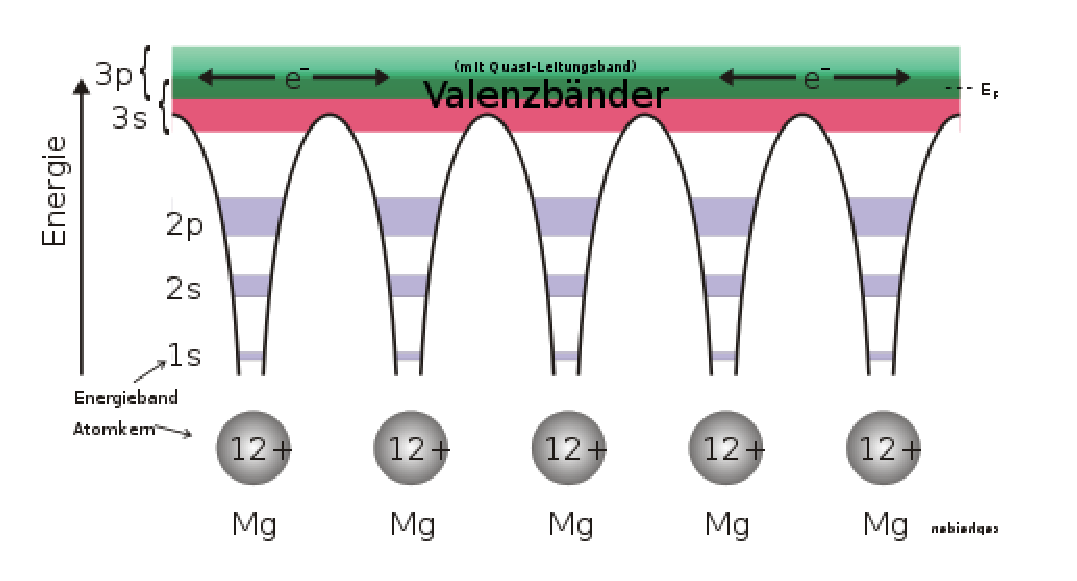
\includegraphics[width=0.9\linewidth]{pictures/baendermodell.eps}
\caption{Bändermodell - Potentialtöpfe}
\end{figure}

\textbf{Einteilung anhand der Lage der Bänder:} \\

Ein \textbf{Isolator} hat ein nicht besetztes Leitungsband und eine so große Bandlücke, dass bei Raumtemperatur und auch bei
deutlich höheren Temperaturen nur sehr wenige Elektronen vom Valenz- ins Leitungsband thermisch angeregt werden. Der
spezifische Widerstand eines solchen Kristalls ist sehr hoch.\\

Ähnlich liegen die Verhältnisse bei einem \textbf{Halbleiter}, jedoch ist die Bandlücke hier so klein $(1 eV < E_G < 3 eV)$,
dass sie durch thermische Energiezufuhr überwunden werden kann. Ein Elektron kann ins Leitungsband angehoben werden und ist
hier beweglich. Zugleich hinterlässt es im Valenzband eine Lücke, die durch benachbarte Elektronen aufgefüllt werden kann.
Somit ist im Valenzband die Lücke beweglich. Man bezeichnet sie auch als Defektelektron, Elektronenfehlstelle oder Loch. Bei
Raumtemperatur weist ein Halbleiter dadurch eine geringe Eigenleitfähigkeit auf, die durch Temperaturerhöhung gesteigert
werden kann. \\

Durch Dotierung kann ein Halbleiter gezielt mit Ladungsträgern ausgestattet werden. Der Halbleiterkristall beruht auf einem
Kristallgitter aus 4-wertigen Atomen, die jeweils durch vier Elektronenpaare gebunden sind. Dotierung mit 5-wertigen Atomen
hinterlässt im Gitter ein für die Bindung nicht erforderliches Elektron, das somit nur locker gebunden ist. Mit nur geringer
Energie kann es daher ins Leitungsband angehoben werden und ist hier beweglich. Ein solches Atom nennt man einen
Elektronen-Donator. Der Kristall wird mit beweglichen negativen Ladungsträgern ausgestattet, man spricht von einer
n-Dotierung. Zugleich bleibt ein positiver Atomrumpf im Gitter zurück. Lässt man den Hintergrund der neutralen Grundsubstanz
außer Betracht, so hat man eine positive feste und eine negative bewegliche Ladung ins Gitter eingebracht. Energetisch liegt
ein Donator knapp unterhalb des Leitungsbandes, da wegen der schwachen Bindung des „zusätzlichen“ Elektrons wenig Energie zur Anregung ins Leitungsband benötigt wird. \\

Dotierung mit 3-wertigen Atomen führt zu einer ungesättigten Bindung, in der ein Elektron fehlt. Dieses kann mit geringem
Energieaufwand aus einer anderen Bindung gerissen werden. Ein solches Atom nennt man einen Elektronen-Akzeptor, das
energetisch knapp oberhalb des Valenzbandes liegt. Es entsteht eine negative ortsfeste Ladung. Zugleich hinterlässt das
Elektron im Kristall eine Lücke, die durch ein anderes Elektron aufgefüllt werden kann, also eine bewegliche
Elektronenfehlstelle. Im Resultat hat man eine negative feste und eine positive bewegliche Ladung eingebracht.
Man spricht dann von p-Dotierung.\\

In einem \textbf{Metall} spricht man meist nicht von Leitungs- bzw. Valenzband. Bei einwertigen Metallen ist das höchste
besetzte Energieband zur Hälfte aufgefüllt. Bei mehrwertigen Metallen überlappen sich teilweise Energiebänder. Elektronen
können daher beim Anlegen von beliebig kleinen elektrischen Feldstärken in einen höheren Energiezustand wechseln (sich
sozusagen frei bewegen) und zum elektrischen Strom beitragen, deswegen sind Metalle gute elektrische Leiter. Eine
Temperaturerhöhung führt im Allgemeinen zur Verringerung der Leitfähigkeit des Kristalls, da die erhöhte Streuung der
Elektronen eine niedrigere mittlere Geschwindigkeit bedingt. Das Ferminiveau liegt bei Metallen bzw. Halbmetallen
innerhalb des höchsten besetzten Bandes bzw. im Überlappungsbereich der Bänder.

\subsubsection{Indirekte Halbleiter}
Indirekte Halbleiter nennt man Halbleiter welche eine indirekte Bandlücke besitzen.
Bei einer indirekten Bandlücke ist das Minimum des Leitungsbandes gegenüber dem Maximum des Valenzbandes auf der $\vec{k}$-Achse verschoben, das heißt der kleinste Abstand zwischen den Bändern ist versetzt. Die Absorption eines Photons ist nur bei einer direkten Bandlücke effektiv möglich, bei einer indirekten Bandlücke muss ein zusätzlicher Quasiimpuls beteiligt werden, wobei ein passendes Phonon erzeugt oder vernichtet wird. Dieser Prozess mit einem Photon allein ist aufgrund des niedrigen Impulses des Lichts wesentlich unwahrscheinlicher, das Material zeigt dort eine schwächere Absorption.

\subsubsection{Extrinsische Halbleiter}
Von einem extrinsischen Halbleiter spricht man wenn die Leitung im Halbleiter vorwiegend durch die der Dotierung zugehörigen Ladungsträger geschieht. Wird die Ladung dagegen hauptsächlich von den eigenen, also den Ladungsträgern die nicht durch die Dotierung entstanden sind getragen so spricht man von einem intrinsischen Halbleiter.

\subsubsection{Spektrometer}
Ein Spektrometer ist ein Instrument zur Messung eines Spektrums, also der Wellenlängenabhängigen Intensität. In unserem Fall handelt es sich um ein optisches Spektrometer welches mittels der Richtungsaufspaltung durch Beugung an einem optischen Gitter arbeitet.

\subsubsection{Lock-In Verstärker}
Bei der Methode des Lock-In Verstärkers wird dem zu messenden Signal ein Referenzsignal bekannter Frequenz aufmoduliert.
Dies geschieht durch das zerhacken des Lichtstrahls (Chopper). Hierbei wird die Orthogonalität von
Sinus und Kosinus ausgenutzt:
\begin{align}
 \int \limits_{-\pi} \limits^{\pi} sin(\omega_1 t)sin(\omega_2 t) dt = \begin{cases} 0 \textnormal{ für } \omega_1\neq\omega_2\\ \pi \textnormal{ für } \omega_1 = \omega_2\end{cases}
\end{align}

Durch den Lock-In Verstärker werden alle Frequenzen die nicht dem Referenzsignal entsprechen, und somit jegliches Rauschen, herausgefiltert. \\

Wichtig ist das Messignal und Referenz genau in Phase sind da sonst die Amplitude des Integrals sinkt oder verschwindet.

\subsection{Haynes- und Shockley-Experiment}

In diesem Experiment soll die Beweglichkeit $\mu$, die Lebensdauer $\tau$ sowie die Diffusions-Konstante positiver Ladungen in Germanium gemessen werden. Historisch handelt es sich um das erste Experiment welches die Bewegung freier Ladungsträger in Halbleitern direkt sichtbar macht. Alle vorherigen Experimente diesbezüglich nutzten den Halleffekt um die Beweglichkeit dieser zu bestimmen.
Durch einen Laserpuls wird in einer Germaniumprobe eine Ladungsträger-Wolke erzeugt. Die Fortbewegung dieser Wolke in einem elektrischen Feld wird mit einem Oszilloskop beobachtet.

\subsubsection{Ladungsträger in Halbleitern}
Betrachtet wird ein Halbleiter im Gleichgewicht, hieraus folgt, dass die Rate an Elektronen-Loch-Paarbildungen gleich der Rate an Rekombinationen von Elektronen und Löchern ist. Einem Elektronen-Loch-Paar kann eine mittlere Lebensdauer $\tau$ zugeschrieben werden. Während dieser Lebenszeit bewegen sich die quasi-freien Teilchen mit der kinetischen Energie $E_{kin}= \frac{3}{2} k T$, so dass der Rekombinationspartner im Allgemeinen nicht der Partner bei der Erzeugung ist. Beim Anlegen eines elektrischen Feldes $\vec{E}$ wird diese Lebenszeit als Beschleunigungszeit wichtig, und es gilt für die mittleren Geschwindigkeiten der Ladungen:
\begin{align}
 \vec{v_n}= \frac{e \vec{E} \tau}{m_n} = -\mu_n \vec{E} ~ ~ \vec{v_p}= \frac{e \vec{E} \tau}{m_p}= -\mu_p \vec{E}
\end{align}

Hier bezeichnen $\mu_n$ und $\mu_p$ die Beweglichkeit der Ladungsträger. Es ist klar, dass die thermische Bewegung nicht zur mittleren Geschwindigkeit beiträgt, da sich diese im Durchschnitt zu Null addiert. Auch die Diffusion kann Einfluss auf den Ladungstransport in Halbleitern nehmen. Die Idee ist, sich die Ladungsträger zunächst neutral vorzustellen. Auch ohne elektrische Abstoßung würde ein Konzentrationsgebiet von Ladungsträgern aufgrund von Stößen auseinander fließen. Führt man die Elektronenkonzentration $n(\vec{x})$, die Loch-Konzentration $p(\vec{x})$ und eine Diffusionskonstante $D_n$ bzw $D_p$ ein, so kann der Ladungsfluss durch Diffusion beschrieben werden als:
\begin{align}
 \vec{j}_{n,diff}=-D_n \vec{\nabla} n ~~~~~~~~~ \vec{j}_{p,diff}=-D_p \vec{\nabla} p
\end{align}

Hiermit kann eine Gleichung für die Elektronen-Stromdichte $\vec{j}_n$ und eine für die Loch-Stromdichte $\vec{j}_p$ gefunden werden:
\begin{align}
\label{Stromdichten}
 \vec{j}_n=- \mu_n n \vec{E} -  D_n \vec{\nabla} n ~~~~~~~~ \vec{j}_p=- \mu_p p \vec{E} -  D_p \vec{\nabla} p
\end{align}

Es ist noch zu erwähnen, dass die Beweglichkeit und die Diffusionskonstante durch die Einstein-Gleichung korreliert sind:
\begin{align}
 D_{n/p}=\frac{kT}{e}\mu_{n/p}
\end{align}

\subsubsection{Herleitung der Ladungsverteilung}

Wir bezeichnen zur Herleitung der Zeitentwicklung der Ladungsträgerwolke die Konzentrationen der Elektronen mit $n$ und die der Löcher mit $p$. Weiter setzen sich diese Konzentrationen aus einer Grundkonzentration $n_o / p_0$ sowie der vom  Laser lokal erzeugten La\-dungs\-kon\-zen\-tra\-tion $\overline{n}(\vec{x})$ bzw $\overline{n}(\vec{x})$ zusammen.
\begin{align}
 n(\vec{x}) = n_0 + \overline{n(\vec{x})}, ~~~~~~p(\vec{x}) = p_0 + \overline{p(\vec{x})}
\end{align}

Der Unterschied zwischen zusätzlichen Löchern und Elektronen gleicht sich, sollte er existieren, nach einer sehr kurzen Zeit (Größenordnung der dielektrischen Relaxationszeit $\tau_{dr}=\epsilon/\sigma \approx 10^{-12}s$) aus. Daher werden wir für unsere Beobachtung (die erst nach dieser Zeit stattfindet) annehmen das diese zusätzlichen Ladungen für Elektronen und Löcher gleich sind, also $\overline{n}=\overline{p}$
 %alter vadder was hat der typ da nur geschrieben ... staatsarbeit fürn arsch mach damit trotzdem weiter
Aus Überlegungen zum thermischen Gleichgewicht wissen wir, dass im Gleichgewicht Erzeugung $G=\frac{n_0}{\tau_0}$ und Rekombination $R=-\frac{n_0}{\tau_0}$ ausgeglichen sind (p analog). Daher wird hier nur die zeitliche Veränderung zusätzlicher Ladungsträger betrachtet (zunächst noch ohne Fluss $\vec{j_{\overline{n}}}$ bzw. $\vec{j_{\overline{p}}}$)
\begin{align}
 \frac{d\overline{n}}{dt}=-\frac{\overline{n}}{\tau_n}~~~~~~~ \frac{d\overline{p}}{dt}=-\frac{\overline{p}}{\tau_p}
\end{align}

Dabei sind $\tau_n$ und $\tau_p$ vorerst nicht als Konstanten zu betrachten, da die Rekombinationszeit des einen Ladungsträgers auch von der verfügbaren Konzentration des jeweils anderen Ladungsträger abhängig ist. Bei dem hier verwendeten p-dotierten Germaniumblock gilt aufgrund der Dotierung $p(\vec{x}) \approx p_0$, somit wird $\tau_p$ hier nun doch zu einer Konstanten. Da sich die Veränderung der zusätzlicher Ladung des einen Ladungsträgers nahezu instantan ($\tau_{dr}$) auf den jeweils andern Ladungsträger überträgt, überträgt sich auch die konstante Rekombinationszeit und es gilt:
\begin{align}
\label{rekombination}
 -\frac{\overline{n}(\vec{x})}{\tau_n}=-\frac{\overline{p}(\vec{x})}{\tau_p},~wenn~~~~~~~~p\gg n
\end{align}

Für die Stromdichten der Ladungsträger folgt mit Gleichung \ref{Stromdichten}:
\begin{align}
 \vec{j}_n=- \mu_n n \vec{E} -  D_n \vec{\nabla} n ~~~~~~~~ \vec{j}_p=- \mu_p p \vec{E} -  D_p \vec{\nabla} p
\end{align}

Weiterhin gilt die Kontinuitätsgleichung. Diese besagt im Normalfall, dass der Massenstrom durch den Rand eines Gebietes gleich der Massenveränderung im Inneren dieses Gebietes ist. Im Fall der hier vorhandenen Ladungsträger muss noch der mögliche Zerfall durch die zusätzliche Rekombinationsrate $-\frac{\overline{n}}{\tau_n}$ bzw. $-\frac{\overline{p}}{\tau_p}$ im Inneren des Gebietes berücksichtigt werden. Damit ergibt die Kontinuitätsgleichung für Elektronen:
\begin{align}
 \frac{\partial n}{\partial t} = - \vec{\nabla} \vec{j_n}- \frac{n-n_0}{\tau_n}=\vec{E}\mu_n \vec{\nabla} n +D_n \Delta n - \frac{n-n_0}{\tau_n}
\end{align}

Dabei haben wir das elektrische Feld innerhalb der Probe als konstant angenommen. Analog gilt für die Löcher:
\begin{align}
 \frac{\partial p}{\partial t} = - \vec{\nabla} \vec{j_p}- \frac{p-p_0}{\tau_p}=-\vec{E}\mu_p \vec{\nabla} p +D_p \Delta p - \frac{p-p_0}{\tau_p}
\end{align}

Diese beiden partiellen Differentialgleichungen sind gekoppelt durch die Notwendigkeit, dass die Rekombinationsrate der zusätzlichen Elektronen und Löcher identisch sein muss (Gleichung \ref{rekombination}). Diese beiden gekoppelten Differentialgleichungen können nach geschickter Addition durch eine Einzige beschrieben und somit gelöst werden. Auch werden zu dieser Beschreibung durch eine einzige Gleichung eine reduzierte Diffusionskonstante $\tilde{D}$ und eine reduzierte Beweglichkeit$\tilde{\mu}$ definiert:
\begin{align}
\tilde{D}&= \frac{\mu_p D_n p + \mu_n D_p n}{n \mu_n + p\mu_p} \\
\tilde{\mu} &= \frac{\mu_n \mu_p (n-p)}{n\mu_n + p\mu_p}
\end{align}

Hier sehen wir die bei dem verwendeten p-dotierten Germanium zulässigen Näherungen nämlich:
\begin{align}
\tilde{D}\rightarrow D_n,~~~ \tilde{\mu}\rightarrow -\mu_n,~\textnormal{wenn} ~~~~~~~~~~p\gg n
\end{align}

Damit kann die Differentialgleichung für diese Ladungsträgerwolke formuliert werden:
\begin{align}
\frac{\partial c}{\partial t} = \tilde{\mu}\vec{E}\vec{\nabla}c + \tilde{D}\Delta c -\frac{c-c_0}{\tau_n}
\end{align}

Diese wird in einer Dimension (unser Fall, da wir nur in einer messen) durch folgende Funktion gelöst:
\begin{align}
c(t,x) = C e^{\frac{t}{\tau_n}} \frac{1}{\sqrt{4\pi\tilde{D}t}} e^{-\frac{(x+\tilde{\mu}Et)^2}{4\tilde{D}t}+C_0}
\end{align}

Diese erinnert stark an eine Gauß-Funktion:
\begin{align}
y(x)=A \frac{1}{2\pi\sigma^2}e^{-\frac{1}{2}(\frac{x-x_c}{\sigma})^2}
\end{align}

Ein direkter Vergleich liefert, dass die Amplitude bzw. Fläche des Signals exponentiell abnimmt, und dieser Zerfall durch die mittlere Lebensdauer der Ladungsträger bestimmt wird.
\begin{align}
A(t)=Ce^{-\frac{t}{\tau_n}}
\end{align}

Des weiteren erkennt man das der Schwerpunkt der Gaußkurve 
\begin{align}
x_c(t)=-E\tilde{\mu} \cdot t
\end{align}

mit konstanter Geschwindigkeit $E\tilde{\mu}$ durch den Halbleiter bewegt. Außerdem lässt die Diffusion die Gaußkurve zerfließen und man sieht leicht:
\begin{align}
\sigma(t)= \sqrt{2\tilde{D}t}
\end{align}

Damit haben wir alles was nötig ist um aus einem Gaußfit die zu messenden Größen Beweglichkeit $\mu_n$, Lebenszeit $\tau_n$ und Diffusionskonstante $D_n$ zu bestimmen.

\subsubsection{Die McKelvey-Korrektur}

Aufgrund der Tatsache das auch während des vorbeifliegens an der Prüfnadel Diffusion stattfindet wird die mittlere Lebensdauer etwas zu groß gemessen. Dieser Effekt ist zwar klein aber relevant. McKelvey erkannte dies wenige Jahre nach der ersten Durchführung des Experiments und führte folgende Korrektur ein. Werden in einer Messreihe mehrere Werte für $\tilde{mu}$ errechnet, so können diese durch
\begin{align}
 \tilde{\mu_0}=\frac{\tilde{\mu}}{\sqrt{x^2+1}-x} \textnormal{mit} ~~~~~x=\frac{2kT}{eEd}(\frac{t}{\tau_n}+\frac{1}{2})
\end{align}

dem wahren Wert $\tilde{\mu_0}$ angepasst werden, d bezeichnet hierbei den Abstand zwischen
Laserinjektion und Nadel.Will man diese Korrektur zur Bestimmung der Diffusionskonstanten $D_n$ mit einbeziehen, kann die McKelvey-Korrektur nicht verwendet werden. Hier empfiehlt es sich eine modifizierte Gauß-Funktion zu verwenden:
\begin{align}
y(x)=A e^{-\frac{x}{\tau}}\frac{1}{2\pi\sigma^2}e^{-\frac{1}{2}(\frac{x-x_c}{\sigma})^2}
\end{align}

\subsection{Halbleiterdetektor}
Wird die Energie eines Photons durch Photo- oder Comptoneffekt in einem
Halbleiter absorbiert, so ensteht eine Vielzahl an Elektron-Loch-Paaren. Etwa
ein Drittel der Energie des Photons regt durch Sekundärstöße des Photo- oder
Comptonelektrons weitere Elektronen in den quasi-freien Zustand des Leitungsbands an.
 Wird an den Halbleiter nun eine Spannung angelegt, so entsteht durch die zusätzliche Ladung ein kurzzeitiges Signal, das proportional 
zur ursprünglichen Energie des Photons ist. Diese Tatsache kann verwendet werden, um die Spektren von
Strahlungsquellen zu vermessen.

\subsubsection{Photoeffekt}
Unter dem äußeren photoelektrischen Effekt (auch Photoeffekt), versteht man das Freisetzen von Elektronen aus einer Metalloberfläche, die von elektromagnetischer Strahlung hinreichend kurzer Wellenlänge getroffen wird.\\

Metalloberflächen geben im negativ geladenen Zustand Elektronen ab, wenn ihre Oberfläche mit Licht bestrahlt wird. Hierbei hängt die kinetische Energie der freiwerdenden Elektronen von der Frequenz des Lichtes ab, aber nicht von dessen Intensität.
Die Freisetzung der Elektronen beginnt sofort bei Einfall des Lichtes. Bei einer Erhöhung der Frequenz des einfallenden Lichtes steigt die kinetische Energie der freiwerdenden Elektronen. Der Effekt tritt erst unterhalb einer bestimmten Wellenlänge welche materialspezifisch ist auf. Die Anzahl der ausgelösten Elektronen ist proportional zur Bestrahlungsstärke.\\

Bis auf die letzte Beobachtung stehen alle gefundenen Zusammenhänge im Widerspruch zur klassischen Vorstellung von Licht als Wellenerscheinung. Die Energie einer Welle hängt danach allein von ihrer Amplitude, nicht jedoch von ihrer Frequenz ab. Der Photoeffekt zeigt somit die Teilcheneigenschaft des Lichtes, ist allerdings kein eindeutiger Nachweis dafür. Semi-klassisch lässt sich der Photoeffekt nämlich auch über die Wechselwirkung einer elektromagnetischen Welle mit einem quantisierten Detektor erklären.

\subsubsection{Comptoneffekt}
Als Compton-Effekt bezeichnet man die Vergrößerung der Wellenlänge eines Photons bei der Streuung an einem Elektron oder einem anderen geladenen Teilchen. Dieser Streuprozess ist nach Arthur Compton benannt und heißt Compton-Streuung.
Compton-Streuung ist der dominierende Wechselwirkungsprozess von Photonen mit Materie für Photonenenergien zwischen etwa 100 keV bis 10 MeV. Ist das Elektron an ein Atom gebunden, so gibt die Compton-Formel die Wellenlängenverschiebung nur noch näherungsweise an, da der Impuls des Elektrons in der Atomhülle zufallsverteilt ist. Den Einfluss des Impulses auf die Winkelabhängigkeit der Energie des gestreuten Photons wird als Dopplerverbreiterung bezeichnet. Sie ist bei niedrigen Energien, großen Streuwinkeln und Atomen mit hoher Kernladungszahl besonders stark ausgeprägt.\\

Bei der Compton-Streuung in Materie wird ein Elektron aus der Atomhülle geschlagen. Somit ist dies ein wichtiger Ionisationsprozess. Der Compton-Effekt kann nicht mit der Vorstellung der klassischen Physik erklärt werden, dass Licht eine elektromagnetische Welle ist. Die Compton-Streuung wird als Stoß zweier Teilchen, Photon und Elektron, beschrieben. Dies zeigt, dass Licht Teilcheneigenschaften hat oder dass Elektronen Welleneigenschaften haben. Denn wenn man Elektronen durch Materiewellen und Licht durch eine elektromagnetische Welle beschreibt, ergibt sich bei ihrer Wechselwirkung ebenfalls der Compton-Effekt.

\subsubsection{MCA}
Ein Vielkanalanalysator (\textbf{M}ulti\textbf{C}hannel\textbf{A}nalyser) dient zur Messung von statistisch verteilten Folgen elektrischer Impulse unterschiedlicher Amplitude, um deren Häufigkeitsverteilung zu ermitteln. Anschaulich gesagt "`sortiert"' das Gerät die regellos eintreffenden Impulse nach ihrer Höhe in verschiedene Kanäle. Meistens stammen die Impulse von einem Teilchen- oder Strahlungsdetektor. Die Häufigkeitsverteilung stellt dann das Spektrum der untersuchten Strahlung dar.\\

Im wesentlichen besteht ein MCA aus einem ADC und einem PC.
Der ADC erzeugt zu jedem Eingangsimpuls diejenige ganze Zahl, die dem der Impulshöhe (Amplitude) proportionalen Wert am nächsten kommt. Die Recheneinheit addiert in demjenigen Kanal, dessen Adresse diese Zahl ist, zum dort vorhandenen Inhalt eine Eins. Der Kanalinhalt am Ende der Messung ist dann die Zahl der aufgetretenen Impulse mit Amplituden in diesem Bereich.

\section{Versuchsaufbau}
\subsection{Vermessung der Bandlücke}
Der Aufbau besteht aus einem Spektrometer, dem Halbleiter und einem Pyrodetektor.
Das Spektrometer liefert Licht mit definierter Wellenlänge welches auf den Halbleiter fällt. Durch Messung des Stroms der im Halbleiter bei angelegter Spannung fließt soll die Absorption gemessen werden. Mit dem Pyrodetektor soll die Transmission gemessen werden.\\

Das \textbf{Spektrometer} besteht aus einer Lampe die weisses Licht erzeugt, dieses wird mittels eines Choppers zerhackt (Lock-in Methode). Anschließend wird es, nach durchlauf einer Linse ($F = 100mm$) zur paralellisierung, an einem drehbaren optischen Gitter reflektiert um schließlich durch eine Blende auf den Halbleiter zu treffen. Zur Drehung wird ein Motor verwendet. Geschwindigkeit und Drehsinn sind wählbar. Der Drehwinkel wird vom Computer erfasst.\\

Der \textbf{Pyrodetektor} besteht aus einem Plattenkondensator, in den als Dielektrikum ein Lithium-Tantalat-Blättchen eingebracht wurde. Durch die vom Chopper erzeugten Lichtpulse ändert sich die Dielektrizität des Kondensators was in einer wechselnden Spannung resultiert welche gemessen werden kann.\\

Um ein möglichst "`sauberes"' Signal zu erhalten wird ein Lock-In Verstärker werwendet.
Die verwendete Referenzfrequenz ist die des Choppers (ca. $70Hz$). Die Phasenbeziehung ist fest eingesetellt und lässt sich nicht verändern.

\subsection{Haynes- und Shockley-Experiment}
Durch einen Lichtleiter, welcher verschiebbar über einer Germaniumprobe monitert ist, wird ein Laserpuls auf die Probe geführt.
Der Laserpuls erzeugt eine konzentrierte Ladungsträgerwolke in der Probe. Durch anlegen einer Spannung an die Probe bewegt sich die Wolke. Mit eine Tastspize die auf der Probe plaziert wird lässt sich auf dem Oszilloskop beobachten wie die Wolke "`vorbeizieht"'. Alle Elektronik zur Laserregelung und Spannungserzeugung befindet sich in einem Gehäuse. An diesem lässt sich Laserintensität und Spannung einstellen. Die Spannung liegt nur gepulst an der Probe an um dieser Zeit zum abkühlen zu lassen.\\

\begin{figure}[H]
\centering
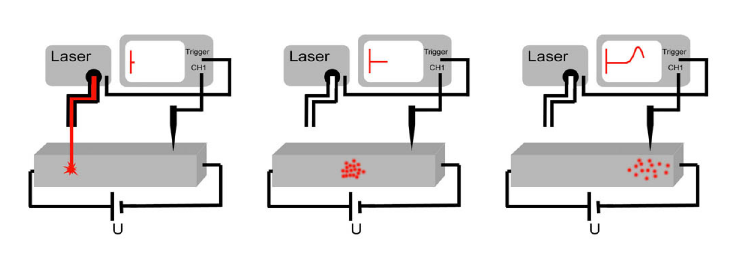
\includegraphics[width=0.9\linewidth]{pictures/haynesAufbau.eps}
\caption{Versuchsablauf, dargestellt zu 3 Zeitpunkten}
\end{figure}

Das zur Verfügung stehende Oszilloskop hat einen USB anschluss über welchen die Messdaten auf einem USB-Stick gespeichert werden können.

\subsection{Halbleiterdetektor}
Zur auswahl stehen eine Siliziumdiode und ein $CdTe$-Kristall zur Verfügung. Der Kristall liegt frei vor, d.h. er muss vor dem Umgebungslicht geschützt werden. Die Detektroren sind beide jeweils mit Elektronik zur Vorverstärkung auf austauschbaren Platinen montiert. Im Gehäuse in dem die jeweilige Platine plaziert wird befindet sich ebenfalls ein weiterer Vorverstärker und ein Shaping Amplifier. Das vom letzterem ausgehende Signal gelangt über einen Vielkanalanalysator MCA8000A in den Computer.

\section{Durchführung}
\subsection{Vermessung der Bandlücke}
Da die Silizium Probe defekt und deshalb nicht mehr vorhanden war mussten wir nur die Germaniumprobe vermessen.
Anfangs stellten wir sicher, dass der Strahlengang korrekt justiert war und machten uns mit dem Motor für das Gitter vertraut.
Da Alle Daten automatisch vom PC aufgezeichnet wurden war jeweils nur der Motor direkt nach der Messung in der richtigen Richtung zu starten und einen Durchlauf von $180^\circ$ abzuwarten. Zwischen den einzelnen Messungen mussten wir des öfteren die Winkelnullstellung wieder tarieren. Ansonsten verlief diser Versuchsteil sehr unproblematisch und schnell.\\

Folgende Messreihen haben wir durchgefüht:
\begin{itemize}
 \item Transmission und Absorption bei voll geöffneter Blende
 \item Untergrund bei voll geöffneter Blende
 \item Transmission und Absorption bei $1cm$-Blendenöffnung
 \item Untergrund bei $1cm$-Blendenöffnung
 \item Wiederholte Messung bei identischer Winkeleinstellung (Fehlerabschätzung)
 \item Lampenspektrum
\end{itemize}

\subsection{Haynes- und Shockley-Experiment}
Nachdem wir ein vernünftiges Signal erhalten hatten namen wir zunächst bei konstantem Abstand und variabler Treiberspannung und dann bei konstanter Treiberspannung und variablem Abstand jeweils zehn Messungen auf.
Die Messung des Abstandes zwischen Nadel und Laser sellte sich dabei als schwierig heraus, warscheinlich wird dieser Fehler alle anderen dominieren.

\subsection{Halbleiterdetektor}

\section{Auswertung}
Zur Auswertung bentzten wir das Datenanalyseframework PyRoot

\subsection{Vermessung der Bandlücke}
Zuerst wurden die Daten vom Untergrund bereinigt und auf die Strahlungsleistung der Lampe normiert:
\begin{align}
 Trans_{real} = \frac{Trans - Untergr_{Trans}}{Lampe} \quad Absorp_{real} = \frac{Absorp - Untergr_{Absorp}}{Lampe}
\end{align}

Da man bei den Mesungen für den Untergrund und das Lampenspektrum nicht die selben $x$-Werte (Winkel bzw. Energien) hat muss man die Daten interpolieren. Wir haben dazu die Punkte der Untergrund- und Spektrumsmessung linear verbunden.

Aus jeder Messung erhält man 2 Plots, einen bei positiven Winkeln und einen bei negativen. Die Fehler auf die gemessene Spannung für die Absorption und Transmission stammen aus der Messung bei konstantem winkel (Standartabweichung). Die Fehler auf die Energie haben wir mit ca. $1^\circ$ also $0,0001~eV$ abgeschätzt. An diese wurden dann jeweils eine konstante Gerade an das Maximum der Apsorptionskurve, eine konstante Gerade an das Minimum der Transmission angepasst. Außerdem wurde an den Bereich des Wendepunks jeder Kurve eine Gerade angefittet. Die $x$-(Energie)-Koordinate des Schnittpunktes liefert dann die Bandlückenenergie. Hier haben wir jeweis das Mittel aus den Beiden Punkten (Transmission / Absorption) genommen. Fehler ist der Fehler des Mittelwerts wobei als Fehler auf die Einzelwerte der Fehler der Steigung genommen wurde da dieser überwiegt. \\
\begin{figure}[H]  
\centering
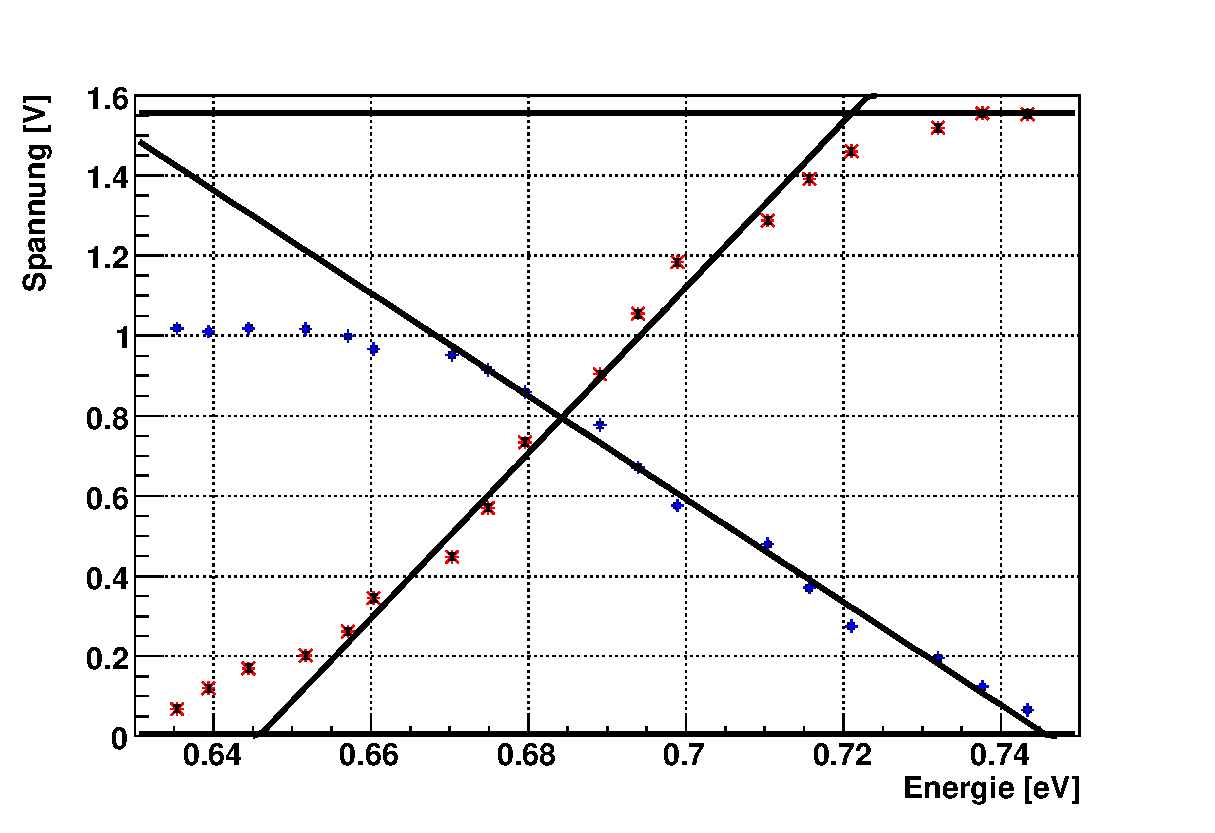
\includegraphics[width=0.9\linewidth]{pictures/bandluecke/grge1.eps}
\caption{Absorption / Transmission bei positiven Winkeln}
\end{figure}

\begin{figure}[H]  
\centering
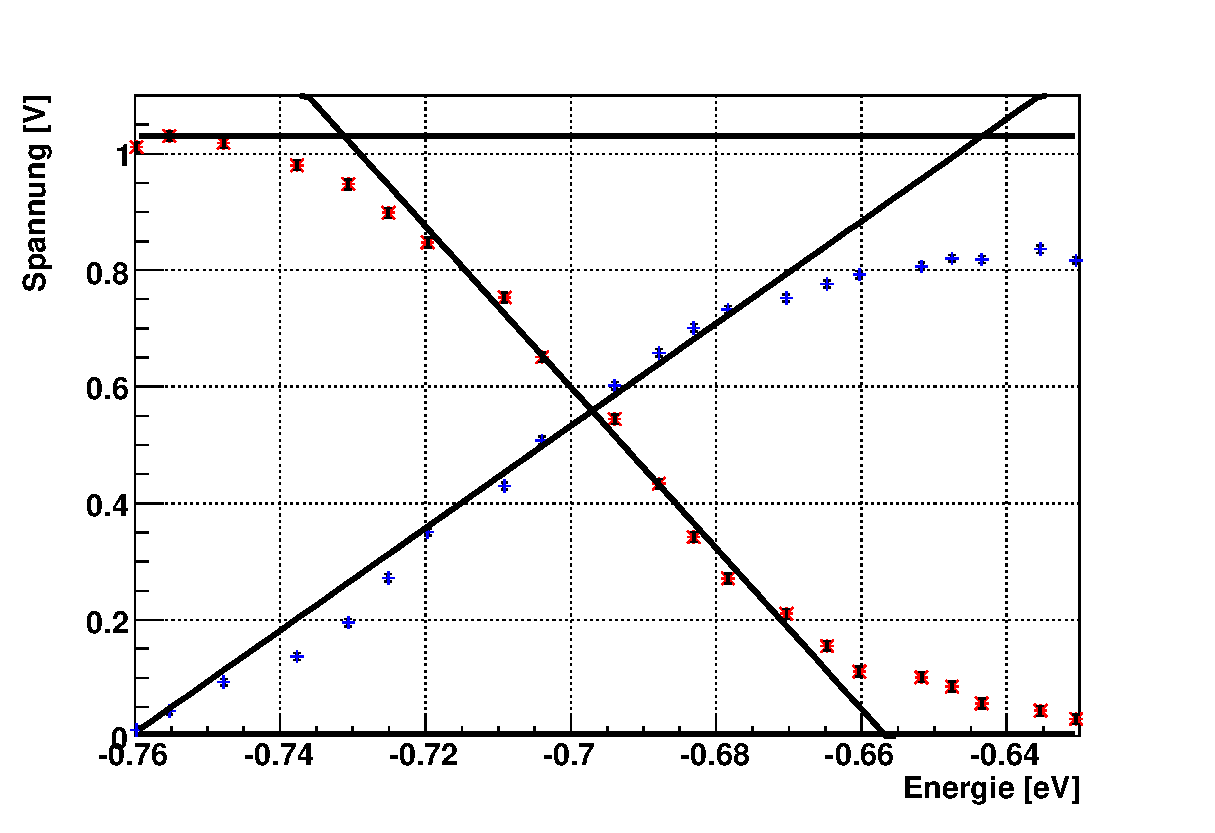
\includegraphics[width=0.9\linewidth]{pictures/bandluecke/grge1b.eps}
\caption{Absorption / Transmission bei negativen Winkeln}
\end{figure}

\begin{figure}[H]  
\centering
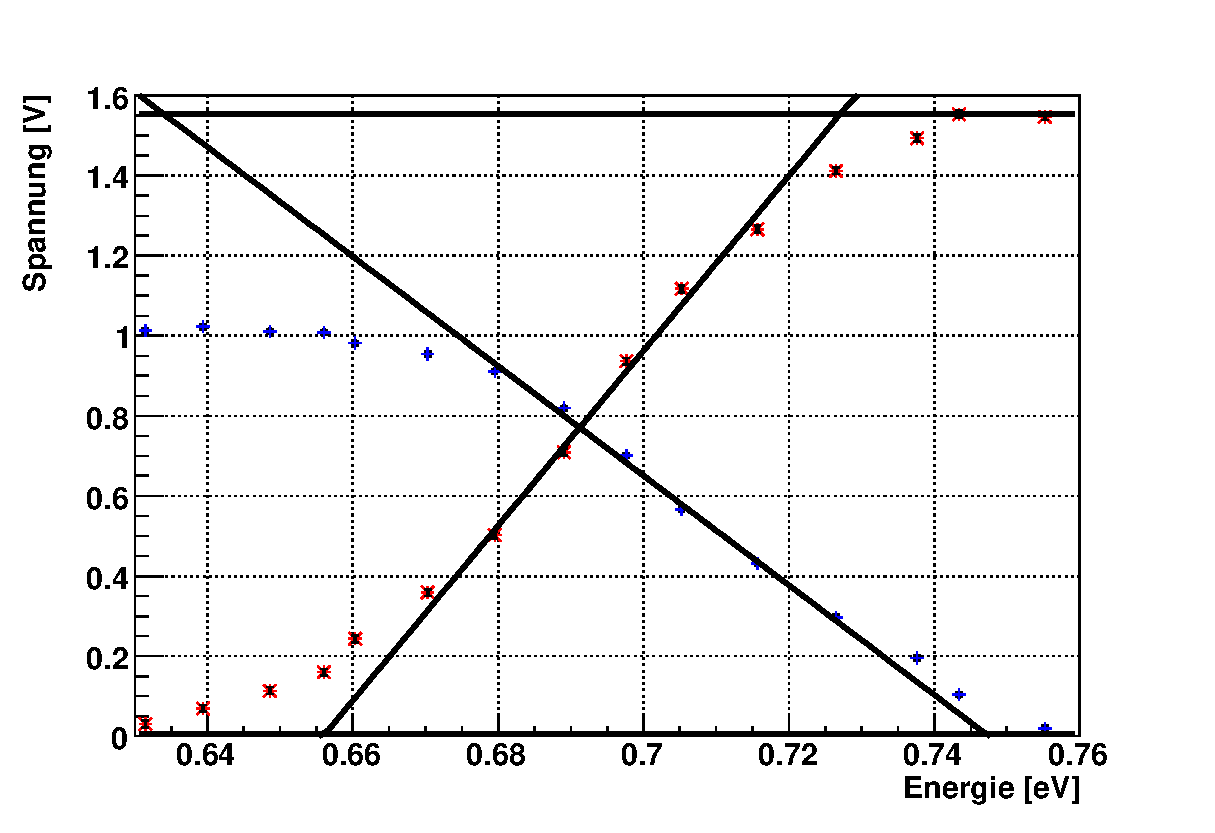
\includegraphics[width=0.9\linewidth]{pictures/bandluecke/grge2.eps}
\caption{Absorption / Transmission bei positiven Winkeln}
\end{figure}

\begin{figure}[H]  
\centering
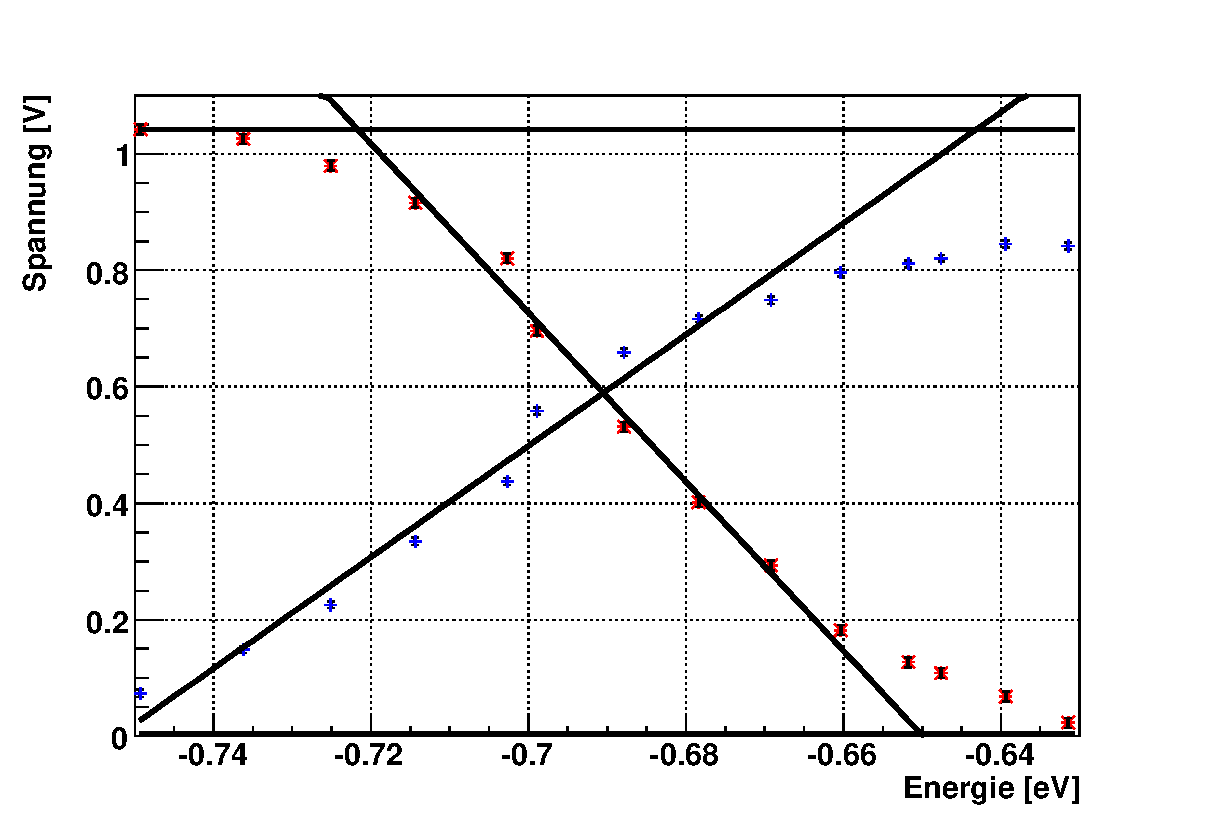
\includegraphics[width=0.9\linewidth]{pictures/bandluecke/grge2b.eps}
\caption{Absorption / Transmission bei negativen Winkeln}
\end{figure}

\begin{figure}[H]  
\centering
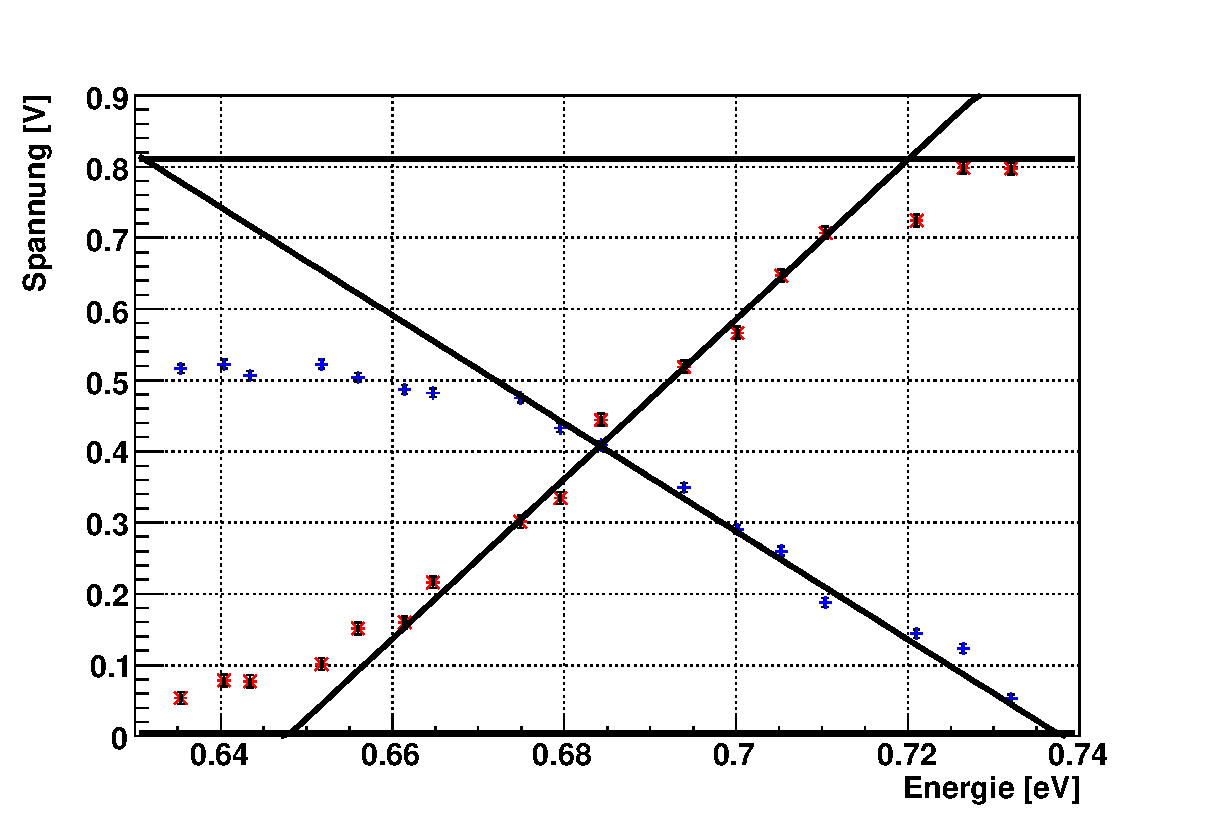
\includegraphics[width=0.9\linewidth]{pictures/bandluecke/grgeb1.eps}
\caption{Absorption / Transmission bei positiven Winkeln, Blende 1cm}
\end{figure}

\begin{figure}[H]  
\centering
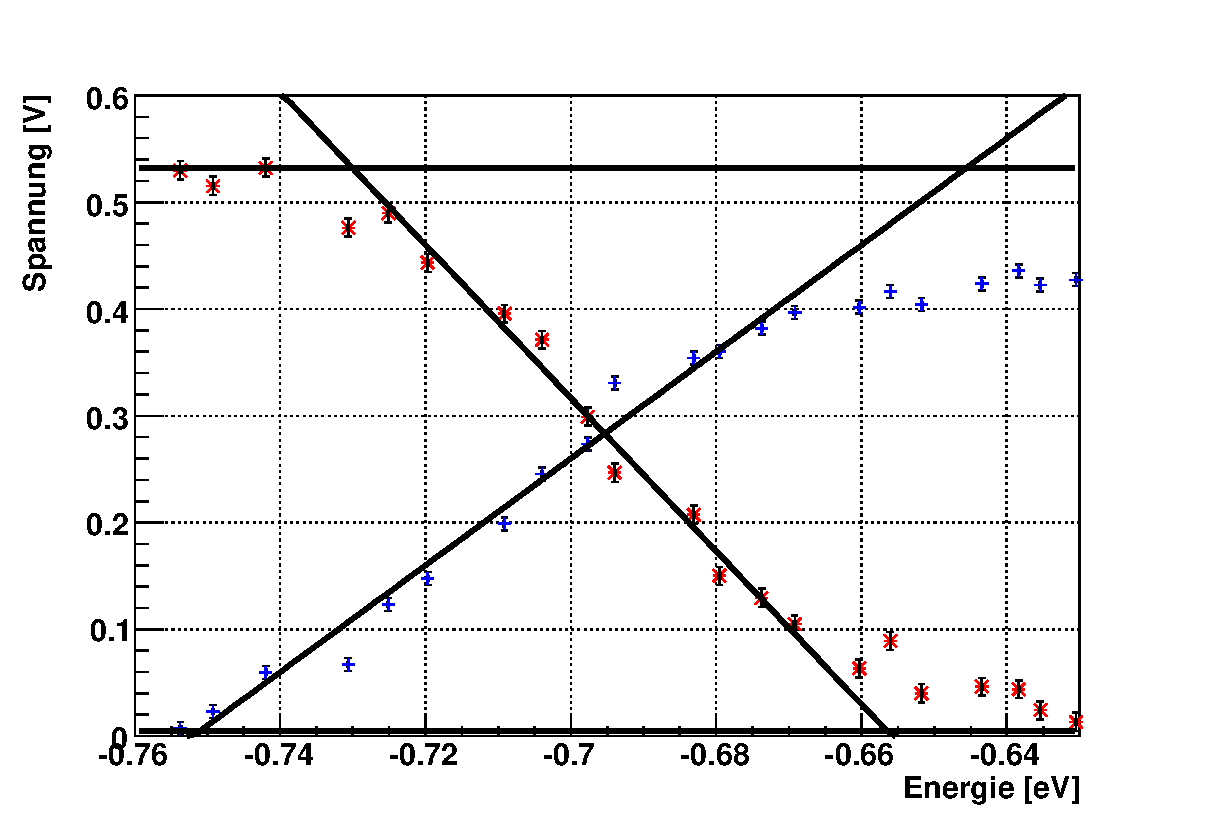
\includegraphics[width=0.9\linewidth]{pictures/bandluecke/grgeb1b.eps}
\caption{Absorption / Transmission bei negativen Winkeln, Blende 1cm}
\end{figure}

\begin{figure}[H]  
\centering
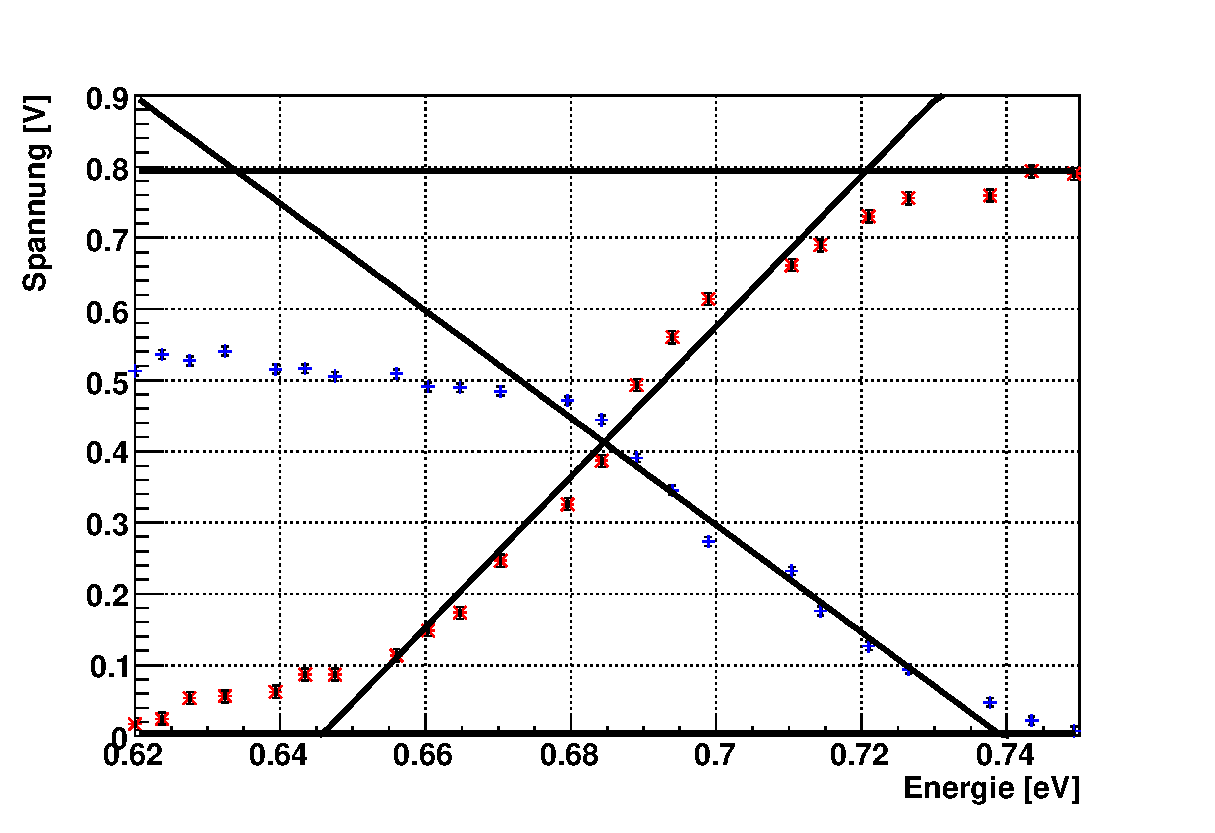
\includegraphics[width=0.9\linewidth]{pictures/bandluecke/grgeb2.eps}
\caption{Absorption / Transmission bei positiven Winkeln, Blende 1cm}
\end{figure}

\begin{figure}[H]  
\centering
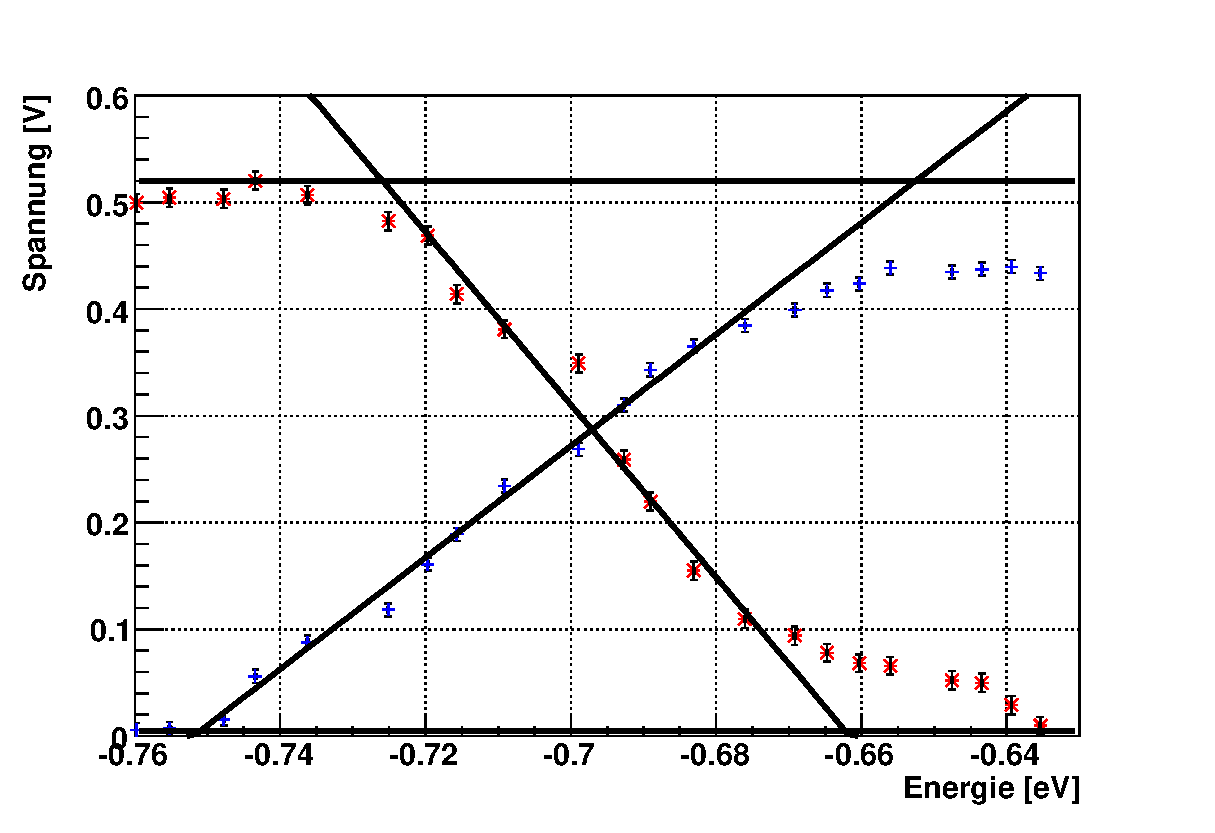
\includegraphics[width=0.9\linewidth]{pictures/bandluecke/grgeb2b.eps}
\caption{Absorption / Transmission bei negativen Winkeln, Blende 1cm}
\end{figure}

Mit den von uns durchgeführten Messungen erhält man somit acht Werte für die Bandlückenenergie. Aus diesen haben wir das gewichtete Mittel berechnet zu:
\begin{align*}
 E_G = 0,741 \pm 0,045
\end{align*}

\subsection{Haynes- und Shockley-Experiment}
\captionfont\footnotesize
Die Mathematik zur Auswertung ist im Kapitel der theoretischen Grundlagen besprochen worden. Die Fehler ergeben sich hier aus den Fits, dh sie werden von Root direkt angegeben. Wir schätzten nur einen Fehler auf die Messung des Osziloskops indem wir die Daten eines konstanten Spannungsverlaufs analysierten und erhielten $5 \cdot 10^{-3}$ als Fehler auf die Spannung (maximale Schwankung) und $1 \cdot 10^{-10}$ als Fehler auf die Zeitmessung (0,1 Prozent, geschätzt).

\subsubsection{Variabler Abstand}
 Wir nahmen zehn Messungen bei variablem Abstand auf. Dieser Lag zwischen 3,8 und 4,7 $mm$, die Treiberspannung betrug 50V. Wir fitteten an jeden Datansatz eine Gausskurve wobei wir den Bereich und die Initialparameter schätzten. Aus den Fits erhielten wir Verläufe der Fitparameter, die wir wieder analysieren konnten. Hierfür benutzten wir folgende Funktionen:
\begin{itemize}
 \item als Gaussfunktion: 
\begin{align*}
U(t) = U_0 + \frac{A}{\sqrt{2\pi \sigma^2}}e^{-\frac{1}{2} \left( \frac{x -x_c}{\sigma}\right)^2 }
\end{align*}
 \item für den Verlauf der Schwerpunkte:
\begin{align*}
x_c(t) = \frac{U}{L} \mu t + x_0
\end{align*}
 \item für den Verlauf der Amplituden:
\begin{align*}
A(t) = C e^{-\frac{t}{\tau}}
\end{align*}
 \item für den Verlauf der Breiten:
\begin{align*}
\sigma(t) = \sqrt{2 D t}
\end{align*}
\end{itemize}

Somit erhielten wir also die Beweglichkeit $\mu$, die Lebenszeit $\tau$ und die Diffusionskonstante $D$ aus diesen letzteren Fits an die Verläufe der Gaussparameter. Diese werden nun dargestellt, es folgen die Ergebnisse dann unsere Gaussfits. Das PyRoot-Skript befindet sich im Anhang.


\begin{figure}[H]  
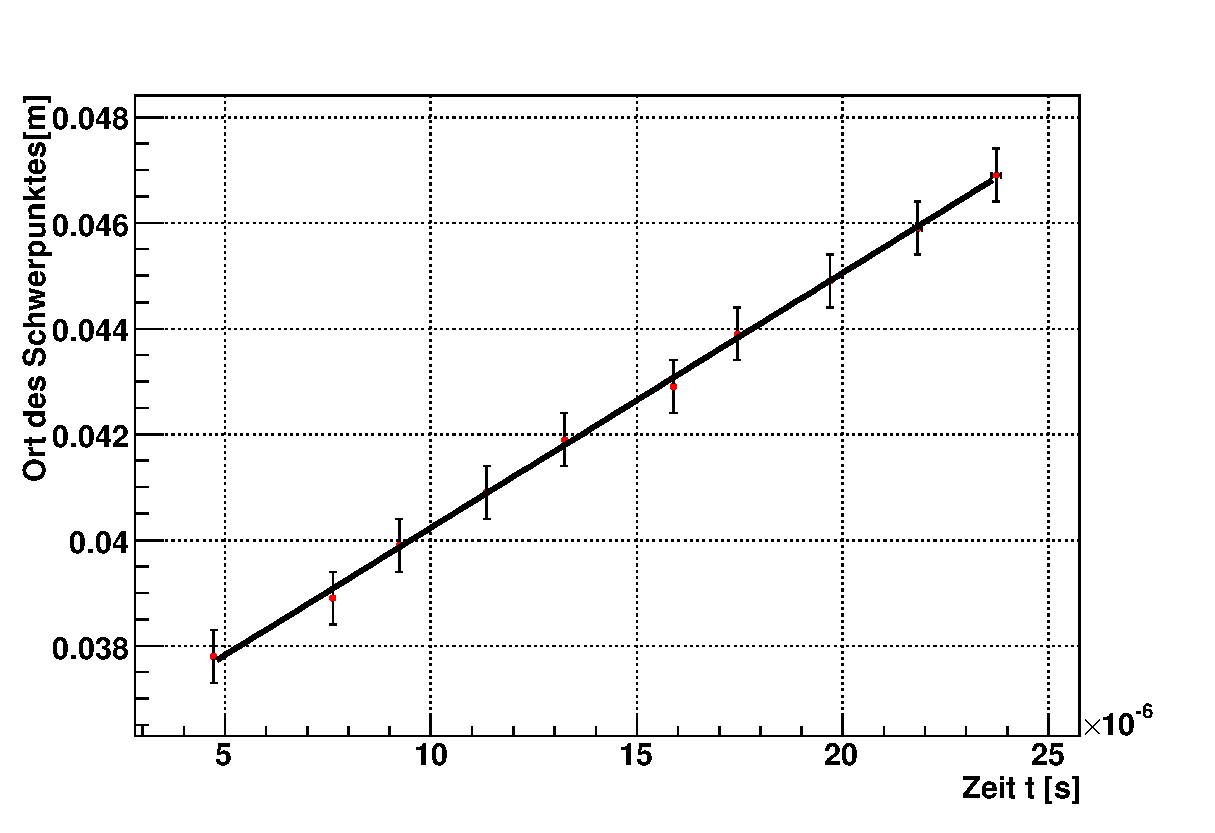
\includegraphics[width=0.9\linewidth]{pictures/varDist/schwerpunkt.eps}
\caption{Verlauf der Schwerpunkte}
\end{figure}

\begin{figure}[H]  
\includegraphics[width=0.9\linewidth]{pictures/varDist/amplitude.eps}
\caption{Verlauf der Amplituden}
\end{figure}

\begin{figure}[H]  
\includegraphics[width=0.9\linewidth]{pictures/varDist/sigma.eps}
\caption{Verlauf der Breiten}
\end{figure}

Aus diesen Fits erhielten wir als Ergebnisse:

\begin{itemize}
 \item Beweglichkeit der Elektronen ~~~~~~~~$\mu = (0,283 \pm 0,016) \frac{m^2}{Vs}$ 
 \item Lebensdauer der Elektronen ~~~~~~~~~~$\tau = (5,22 \pm 0,03) 10^{-5} s $
 \item Diffusionskonstante der Elektronen ~~$D = (5,42 \pm 0,03) 10^{-8} \frac{m^2}{s}$
\end{itemize}


\newpage
Hier unsere Gaussfits, hier ist das Verlaufen der Ladungsträgerwolke mit dem Abstand schön zu erkennen. Unter den Abbildungen ist der Abstand Laser - Nadel angegeben.

\begin{figure}[H]  
\begin{minipage}{0.33\linewidth}
\centering
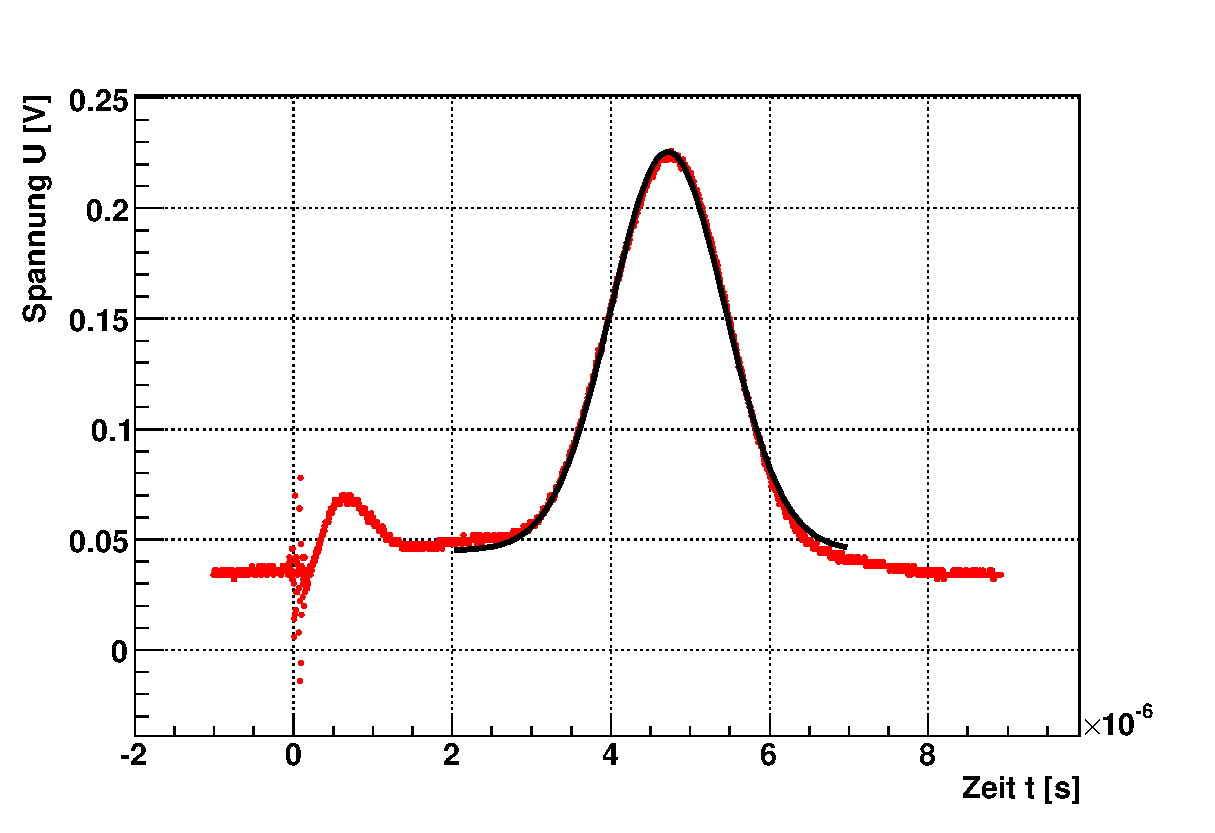
\includegraphics[width=0.9\linewidth]{pictures/varDist/00.eps}
\small{3,78 mm}
\end{minipage}
\begin{minipage}{0.33\linewidth}
\centering
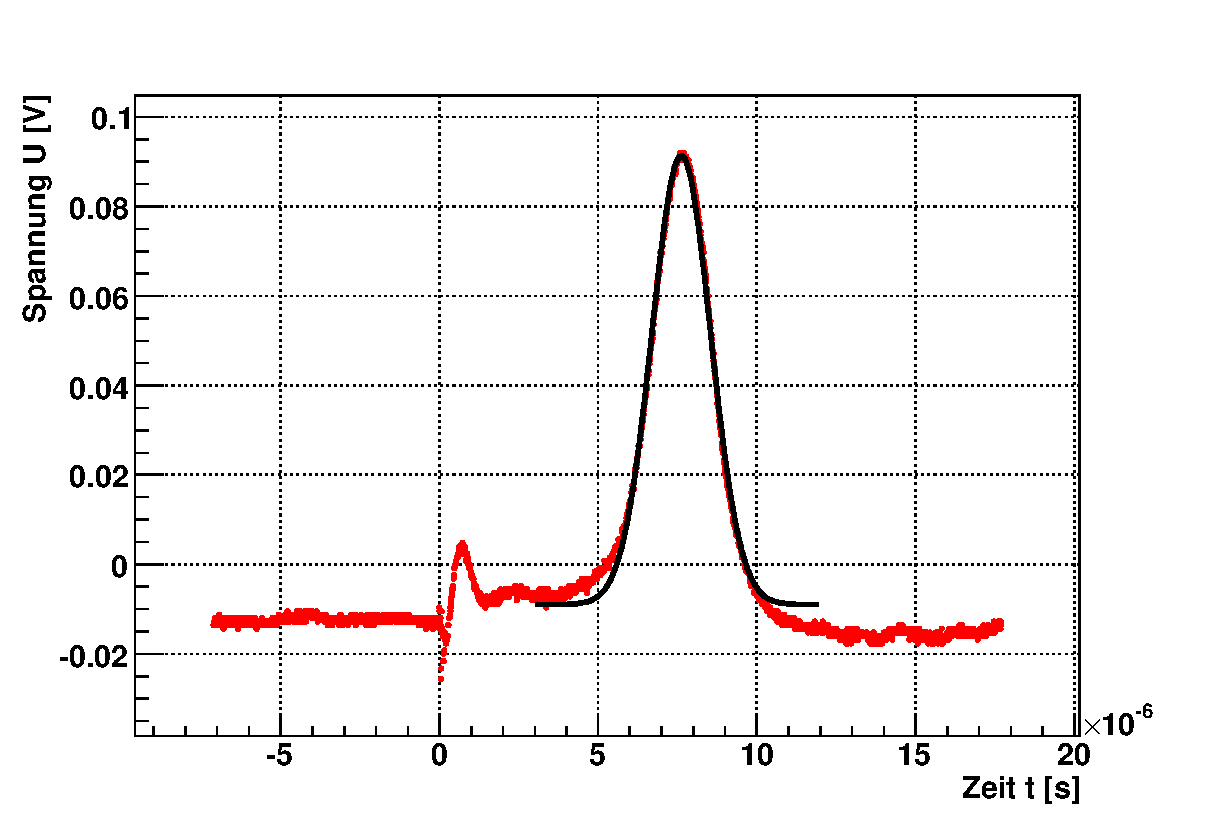
\includegraphics[width=0.9\linewidth]{pictures/varDist/09.eps}
\small{3,89 mm}
\end{minipage}
\begin{minipage}{0.33\linewidth}
\centering 
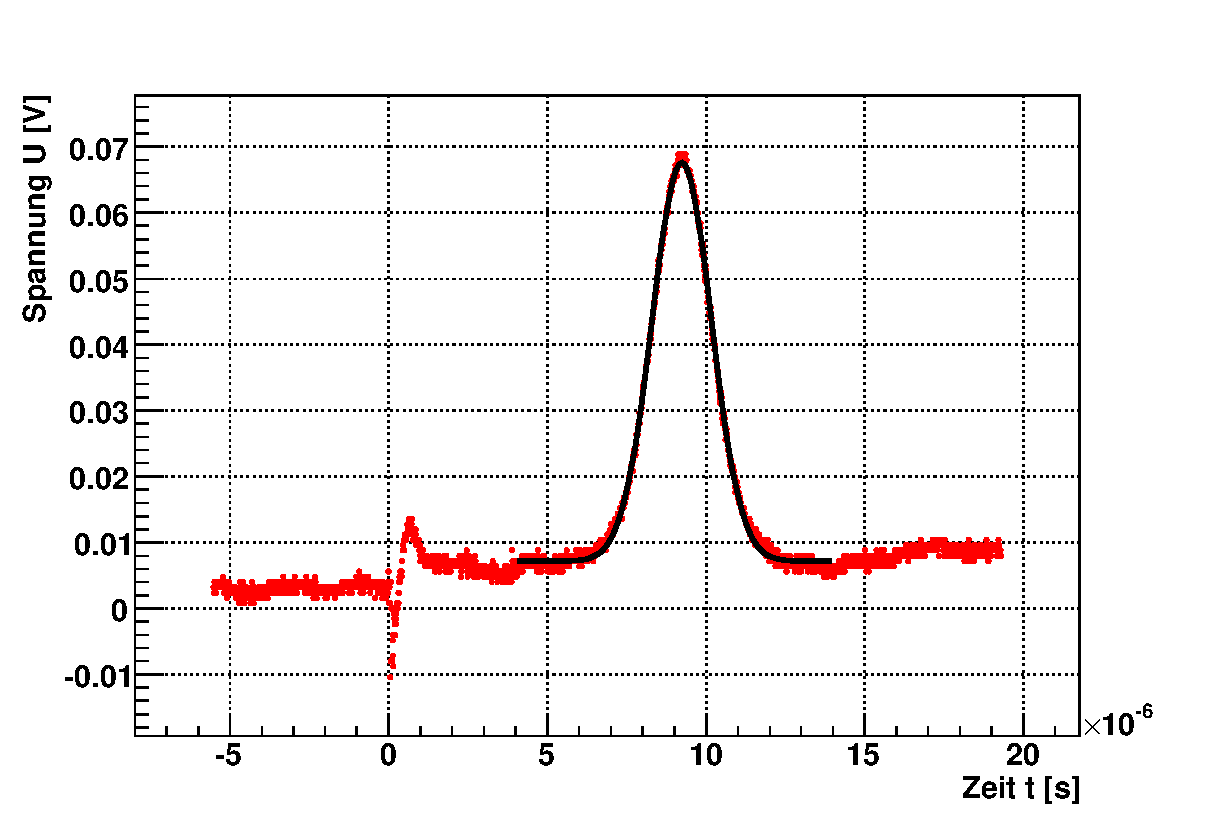
\includegraphics[width=0.9\linewidth]{pictures/varDist/01.eps}
\small{3,99 mm}
\end{minipage}
\end{figure}

\begin{figure}[H]  
\begin{minipage}{0.33\linewidth}
\centering
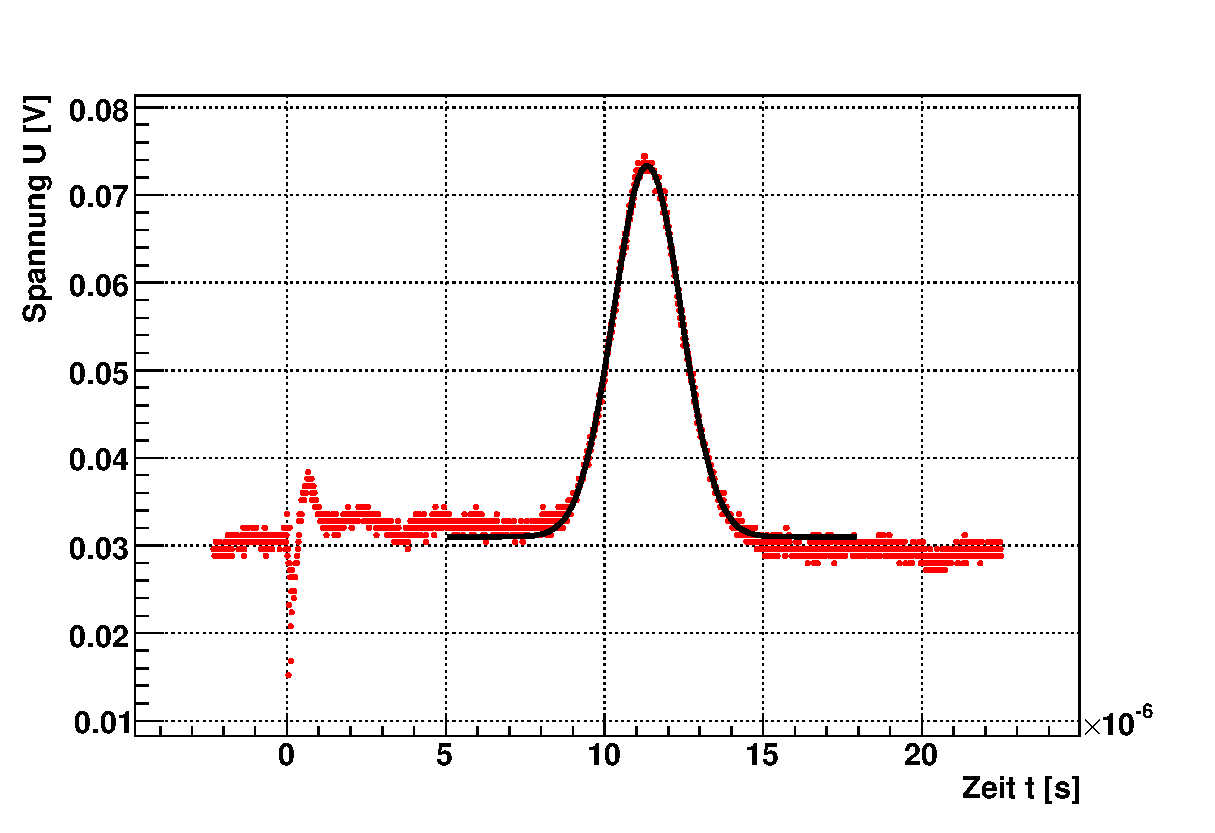
\includegraphics[width=0.9\linewidth]{pictures/varDist/08.eps}
\small{4,09 mm}
\end{minipage}
\begin{minipage}{0.33\linewidth}
\centering
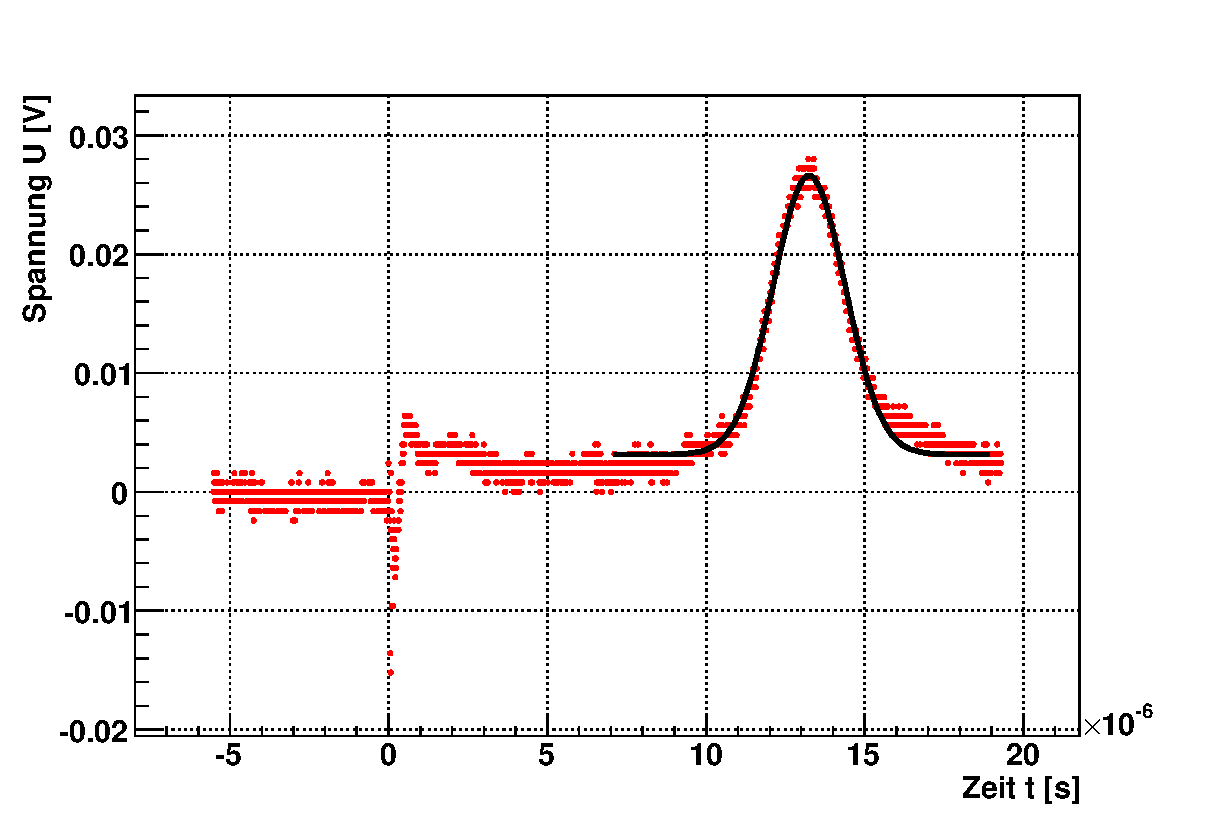
\includegraphics[width=0.9\linewidth]{pictures/varDist/02.eps}
\small{4,19 mm}
\end{minipage}
\begin{minipage}{0.33\linewidth}
\centering 
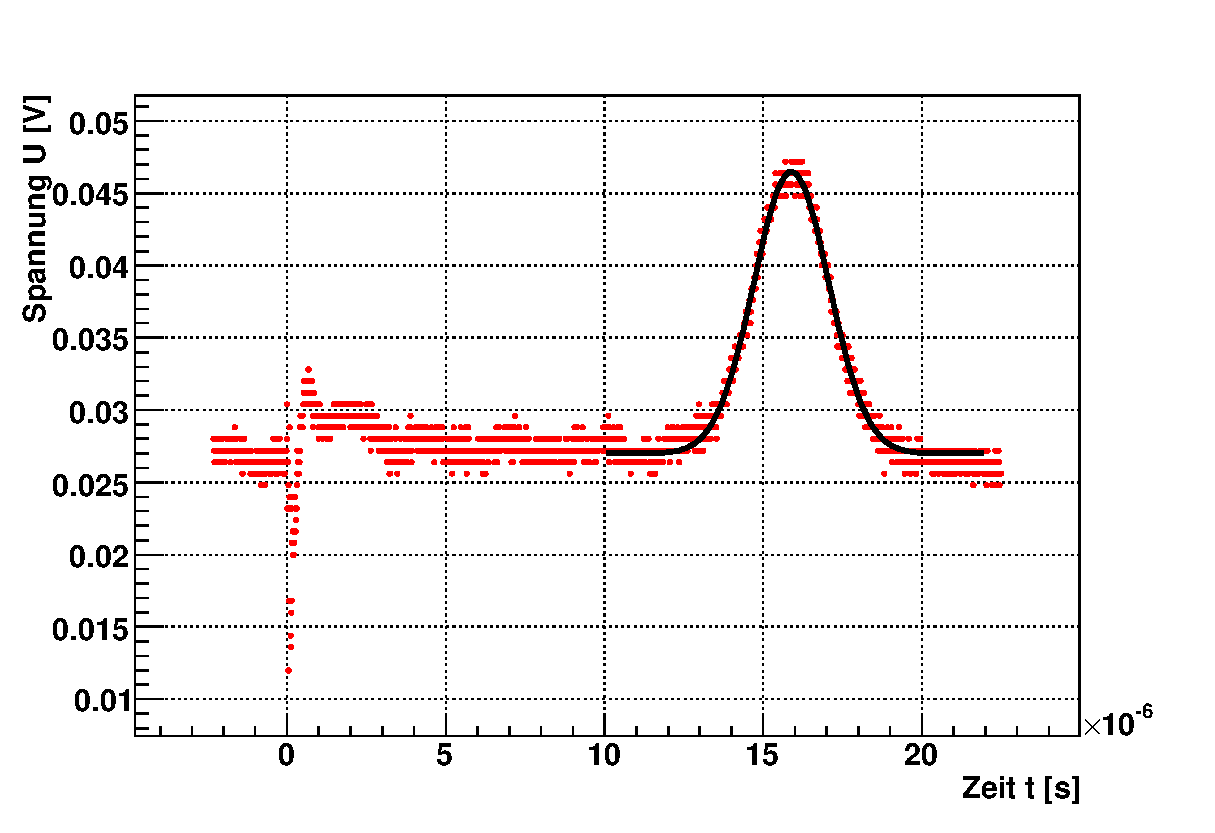
\includegraphics[width=0.9\linewidth]{pictures/varDist/07.eps}
\small{4,29 mm}
\end{minipage}
\end{figure}

\begin{figure}[H]  
\begin{minipage}{0.33\linewidth}
\centering
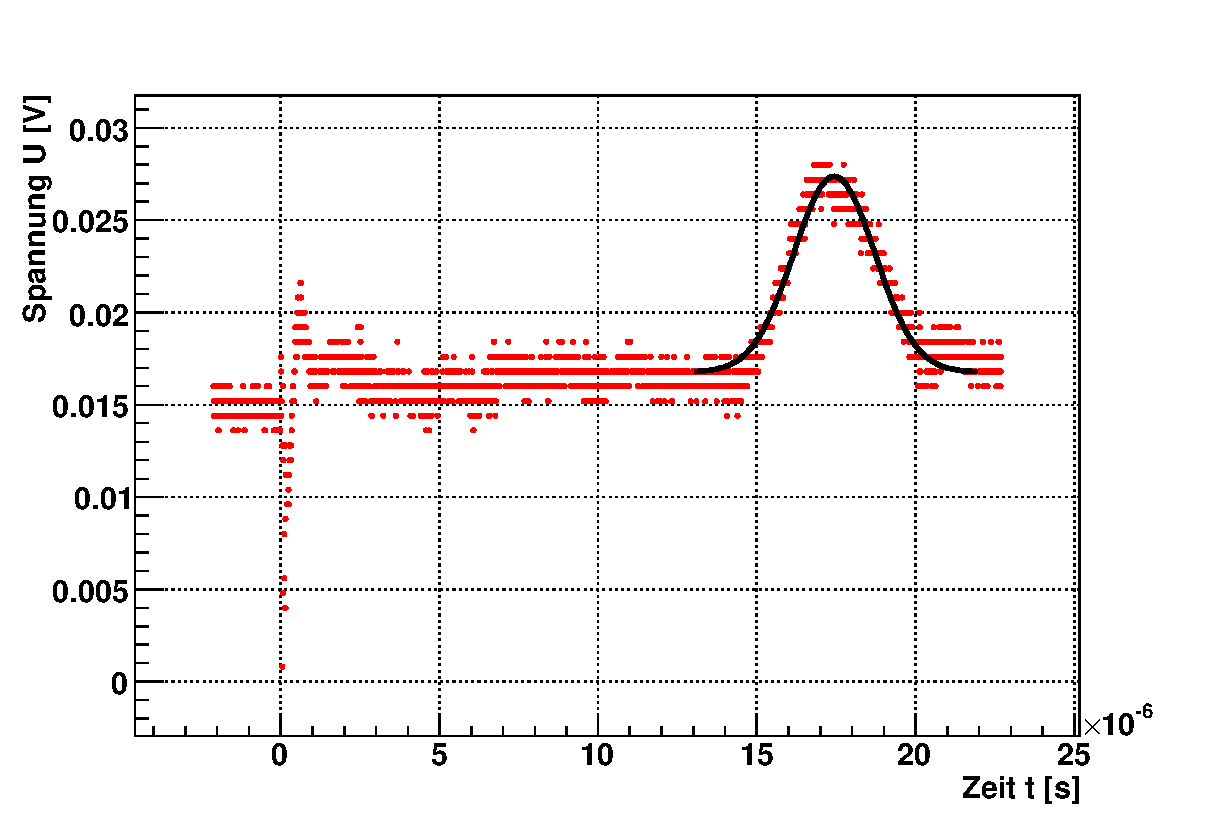
\includegraphics[width=0.9\linewidth]{pictures/varDist/03.eps}
\small{4,39 mm}
\end{minipage}
\begin{minipage}{0.33\linewidth}
\centering
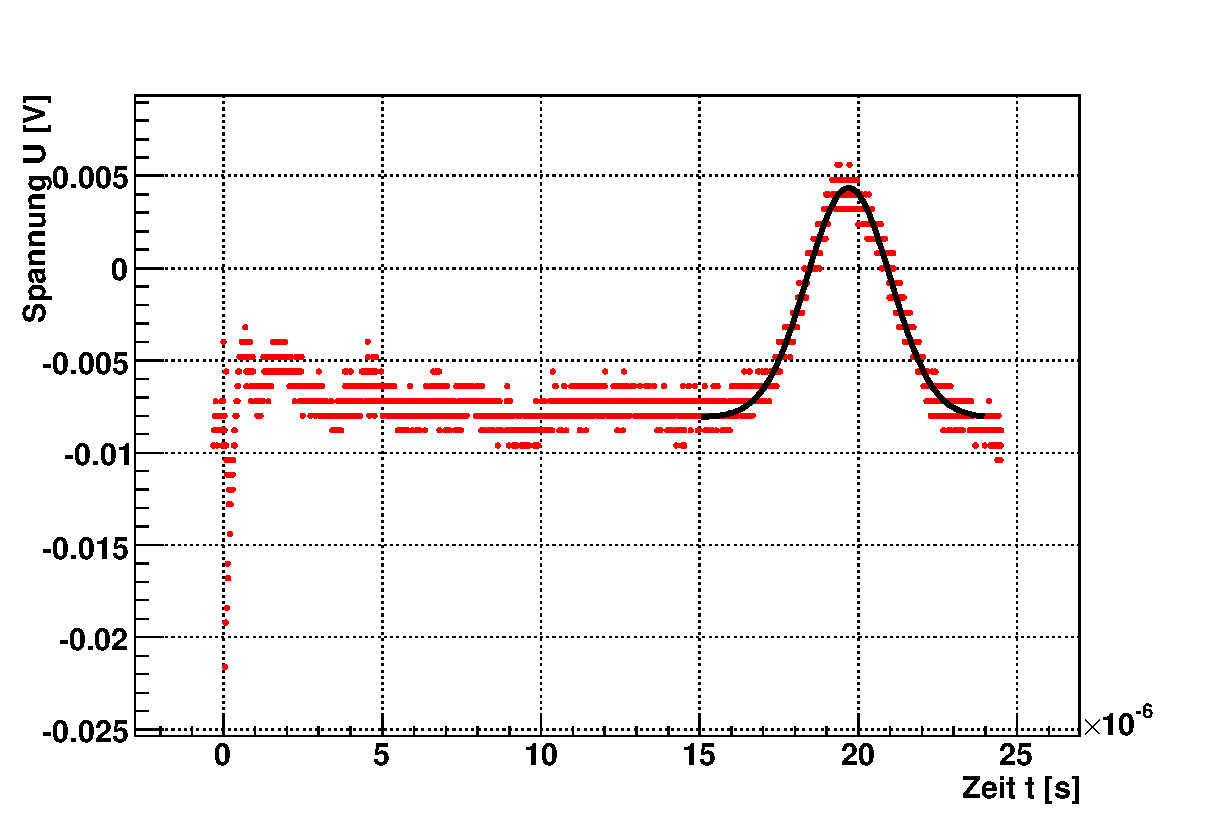
\includegraphics[width=0.9\linewidth]{pictures/varDist/06.eps}
\small{4,49 mm}
\end{minipage}
\begin{minipage}{0.33\linewidth}
\centering 
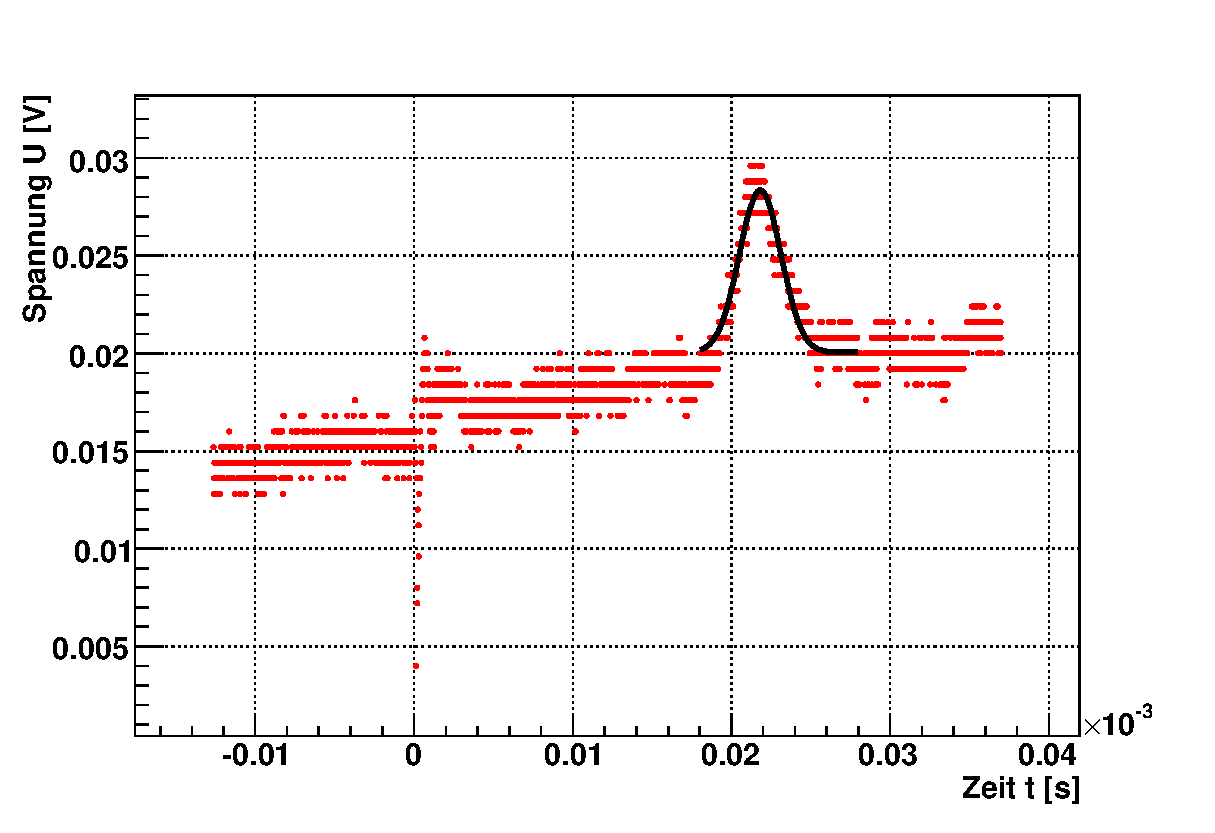
\includegraphics[width=0.9\linewidth]{pictures/varDist/04.eps}
\small{4,59 mm}
\end{minipage}
\end{figure}

\begin{figure}[H]  
\begin{minipage}{0.33\linewidth}
\centering
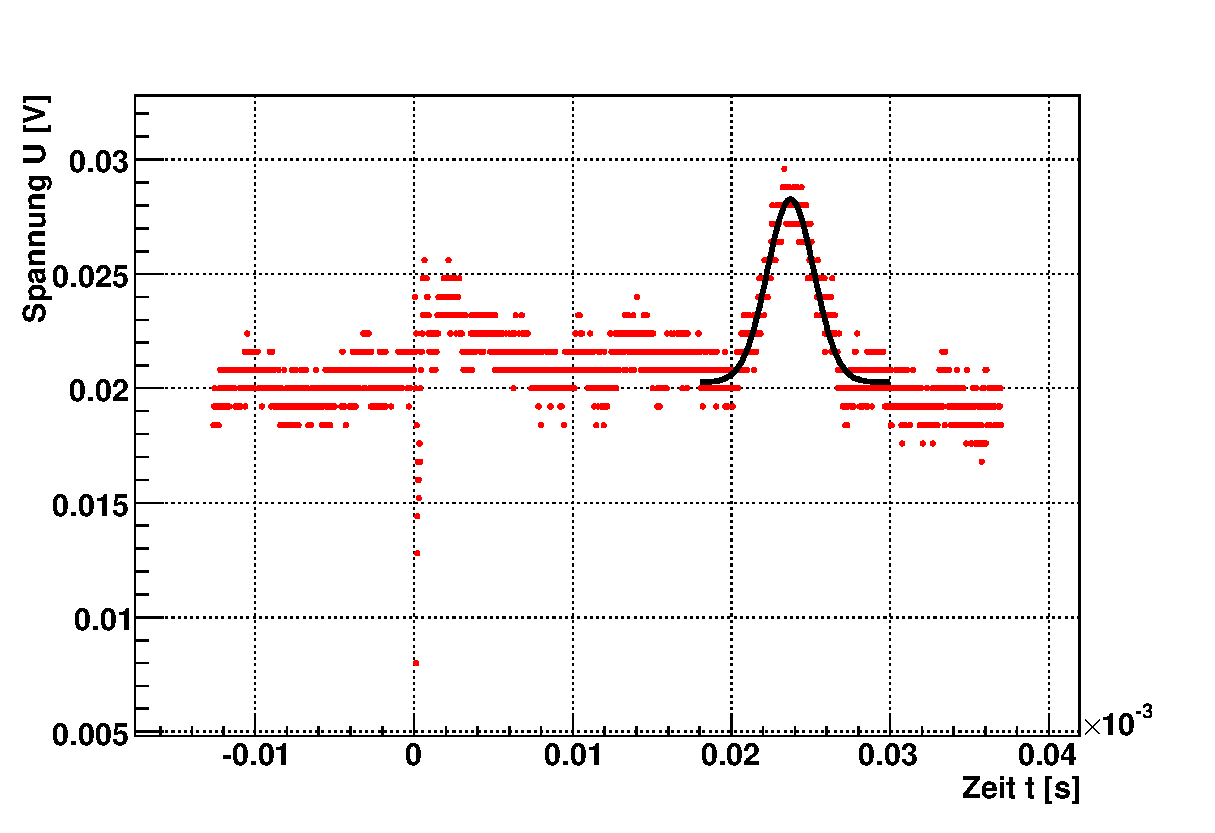
\includegraphics[width=0.9\linewidth]{pictures/varDist/05.eps}
\small{4,69 mm}
\end{minipage}
\begin{minipage}{0.33\linewidth}
\centering
\end{minipage}
\begin{minipage}{0.33\linewidth}
\centering 
\end{minipage}
\end{figure}
\newpage

\subsubsection{Variation des elektrischen Felds}
Hier nahmen wir zwölf Messreihen auf, wobei wir die Treiberspannung zwischen 15,2 V und 51,2 V variierten. Der Abstand lag bei allen Messungen bei 3,98 mm. Zur Auswertung sind hier noch ein paar überlegungen zum Fit der Schwerpunkte zu machen: Da wir den Ort der Messung nicht Verändern gilt:
\begin{align*}
 x_c = E \mu t + x_0 = const. = 3,98 mm
\end{align*}

wobei nun das elektrische Feld E und die Zeit bis zur Schwerpunktsdetektion t variabel sind. Es ergibt sich also:
\begin{align*}
 t = \frac{x_c+x_0}{E \mu} + t_0
\end{align*}

als Fitfunktion an die Daten des Schwerpunktes. Alle anderen Fitfunktionen bleiben unverändert:

\begin{figure}[H]  
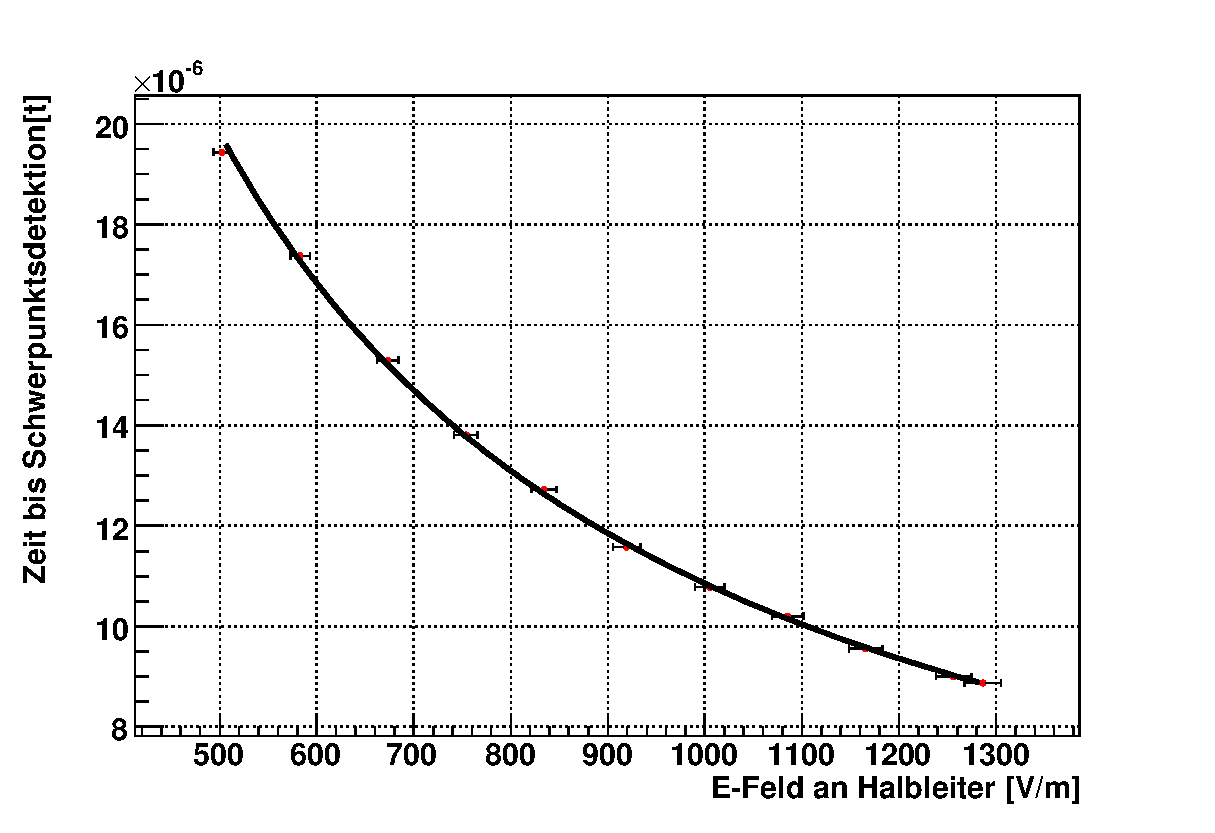
\includegraphics[width=0.9\linewidth]{pictures/varVolt/movabilty.eps}
\caption{Verlauf der Schwerpunkte}
\end{figure}

\begin{figure}[H]  
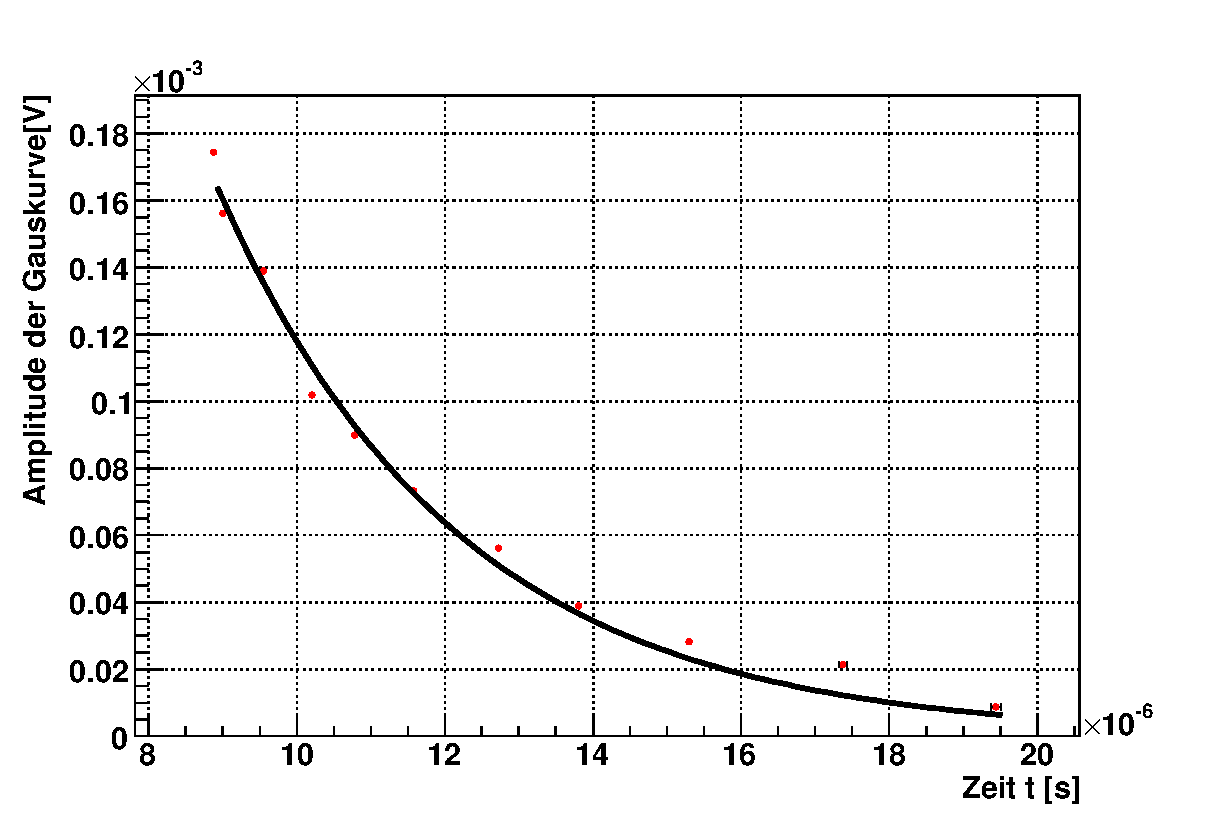
\includegraphics[width=0.9\linewidth]{pictures/varVolt/lifetime.eps}
\caption{Verlauf der Amplituden}
\end{figure}

\begin{figure}[H]  
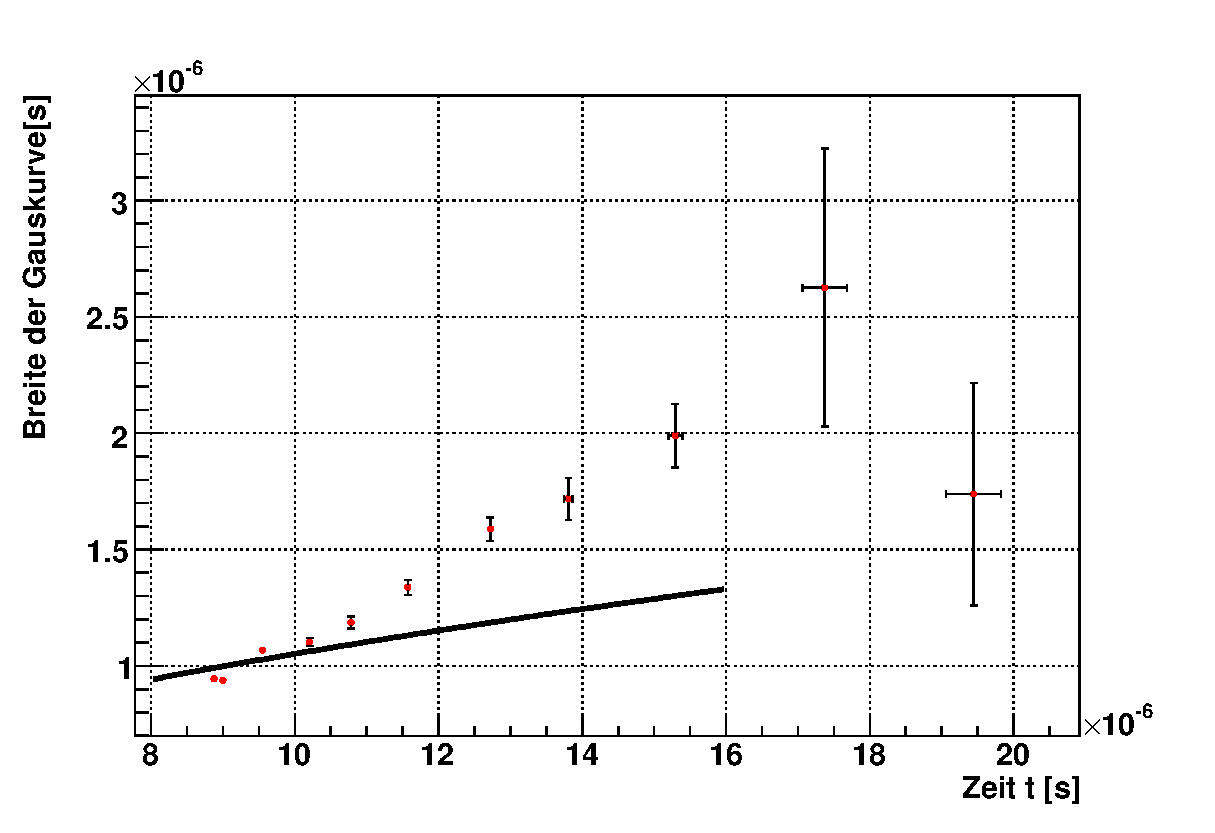
\includegraphics[width=0.9\linewidth]{pictures/varVolt/diffusion.eps}
\caption{Verlauf der Breiten}
\end{figure}
\newpage

Aus diesen Fits erhielten wir als Ergebnisse:
\begin{itemize}
 \item Beweglichkeit der Elektronen ~~~~~~~~~$\mu = (111 \pm 8) \frac{m^2}{Vs}$ 
 \item Lebensdauer der Elektronen ~~~~~~~~~~~$\tau = (3,25 \pm 0,05) 10^{-5} s $
 \item Diffusionskonstante der Elektronen ~~$D = (5,53 \pm 0,06) 10^{-8} \frac{m^2}{s}$
\end{itemize}

Hier die Gaussfits, unter den Abbildungen ist die Treiberspannung angegeben:

\begin{figure}[H]  
\begin{minipage}{0.33\linewidth}
\centering
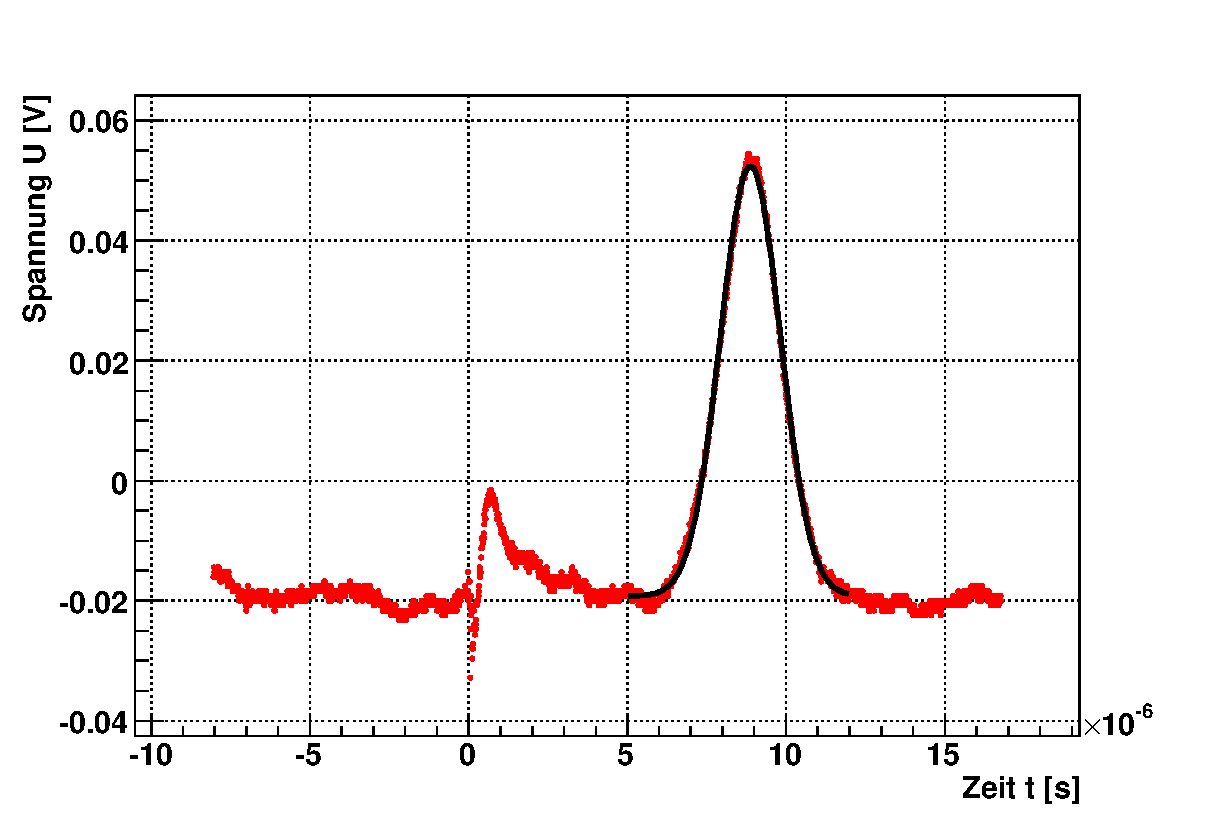
\includegraphics[width=0.9\linewidth]{pictures/varVolt/00.eps}
\small{51,2 V}
\end{minipage}
\begin{minipage}{0.33\linewidth}
\centering
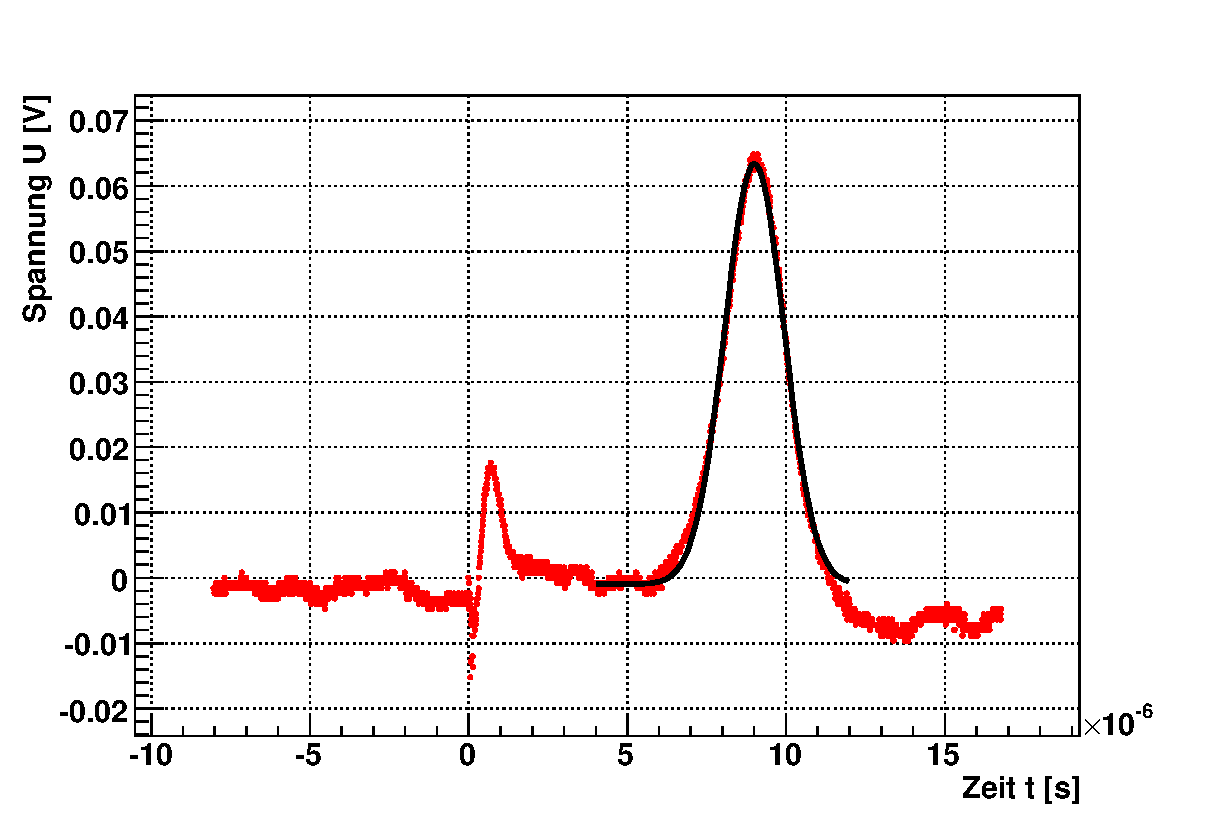
\includegraphics[width=0.9\linewidth]{pictures/varVolt/01.eps}
\small{50 V}
\end{minipage}
\begin{minipage}{0.33\linewidth}
\centering 
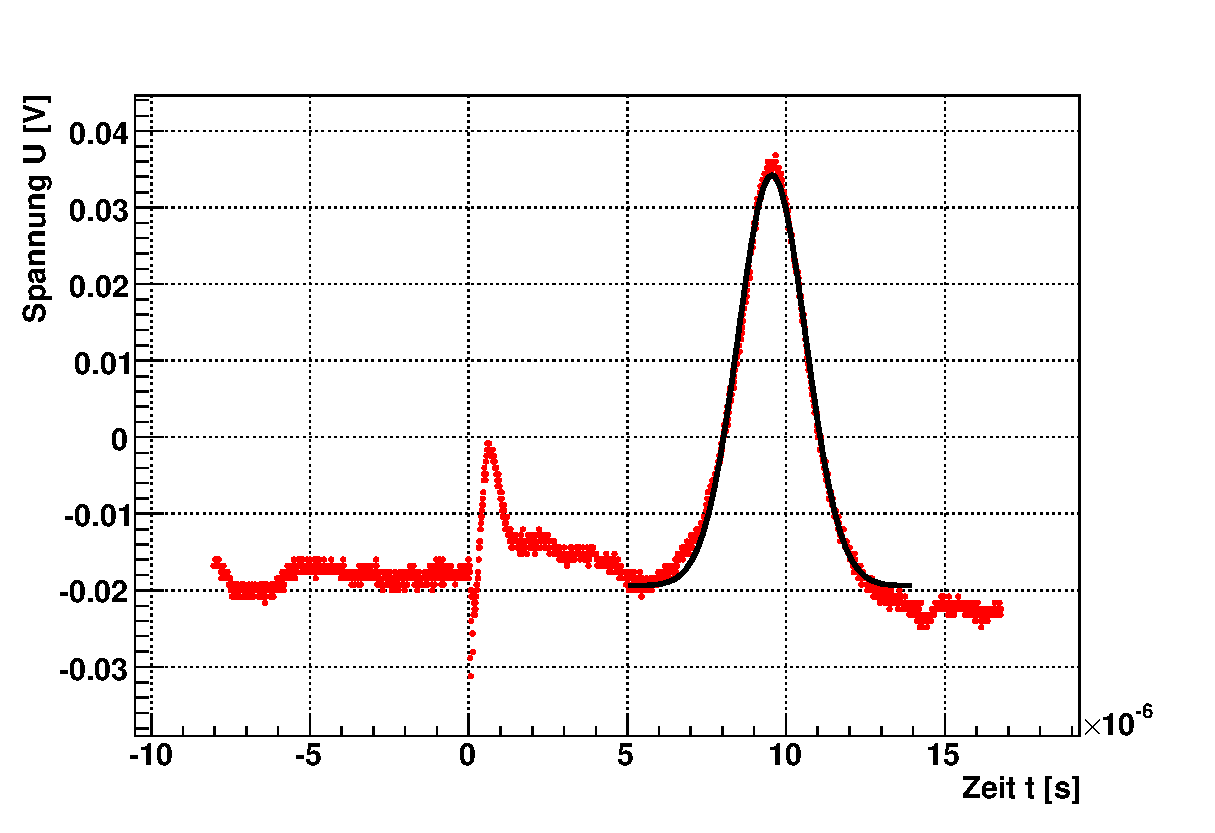
\includegraphics[width=0.9\linewidth]{pictures/varVolt/02.eps}
\small{46,4 V}
\end{minipage}
\end{figure}

\begin{figure}[H]  
\begin{minipage}{0.33\linewidth}
\centering
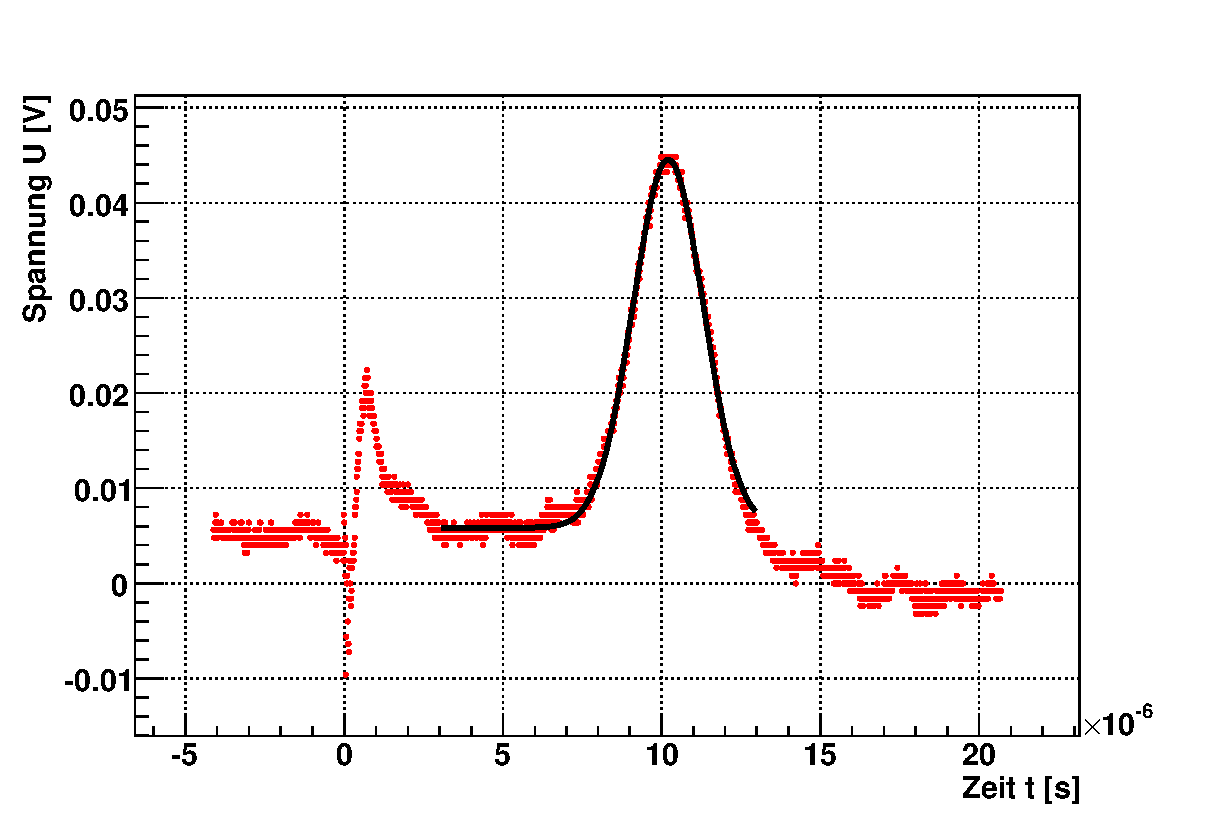
\includegraphics[width=0.9\linewidth]{pictures/varVolt/03.eps}
\small{43,2 V}
\end{minipage}
\begin{minipage}{0.33\linewidth}
\centering
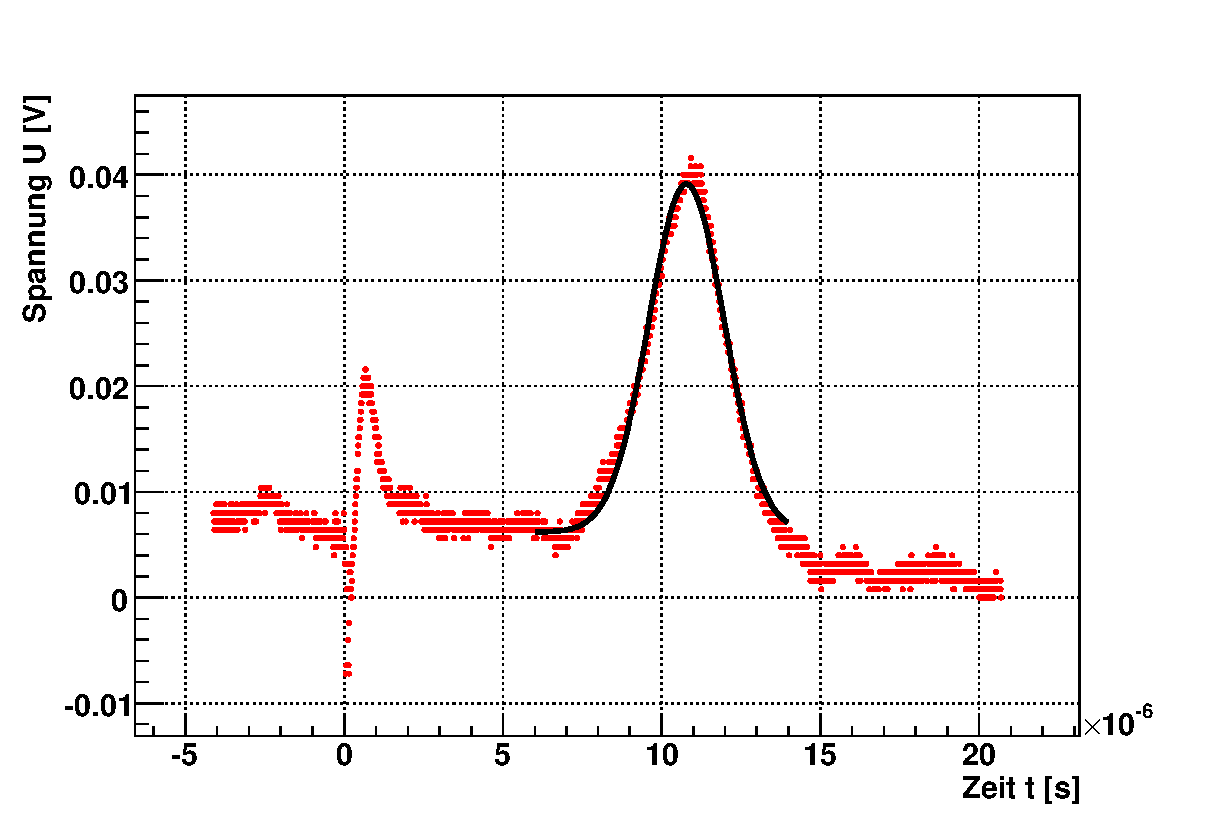
\includegraphics[width=0.9\linewidth]{pictures/varVolt/04.eps}
\small{40 V}
\end{minipage}
\begin{minipage}{0.33\linewidth}
\centering 
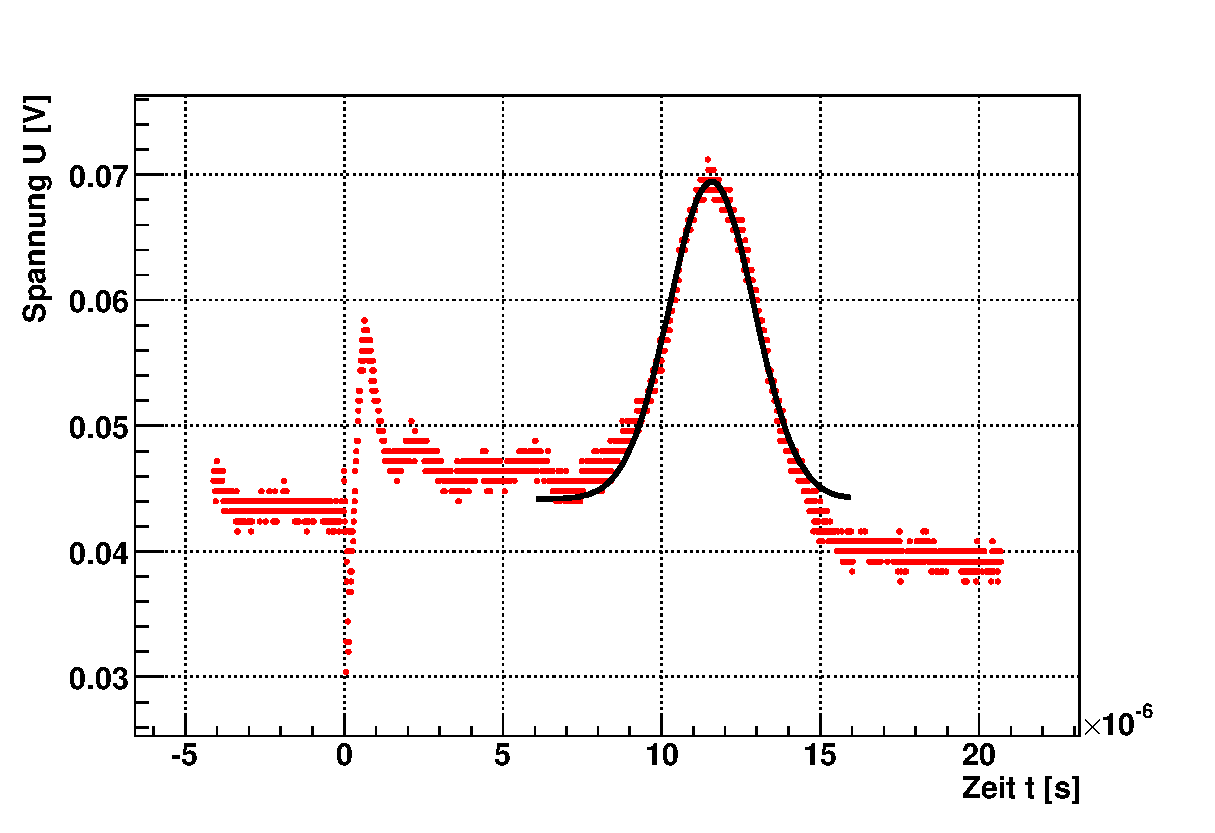
\includegraphics[width=0.9\linewidth]{pictures/varVolt/05.eps}
\small{36,6 V}
\end{minipage}
\end{figure}

\begin{figure}[H]  
\begin{minipage}{0.33\linewidth}
\centering
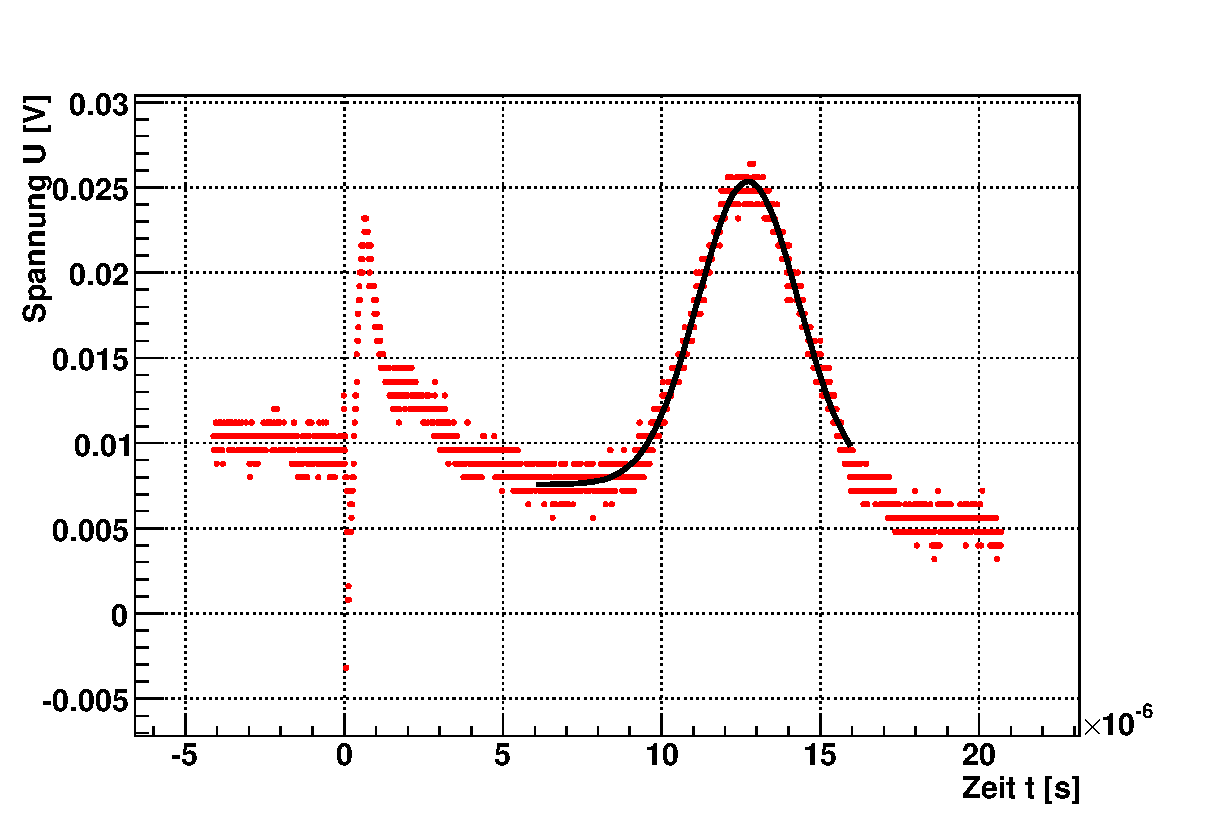
\includegraphics[width=0.9\linewidth]{pictures/varVolt/06.eps}
\small{33,2 V}
\end{minipage}
\begin{minipage}{0.33\linewidth}
\centering
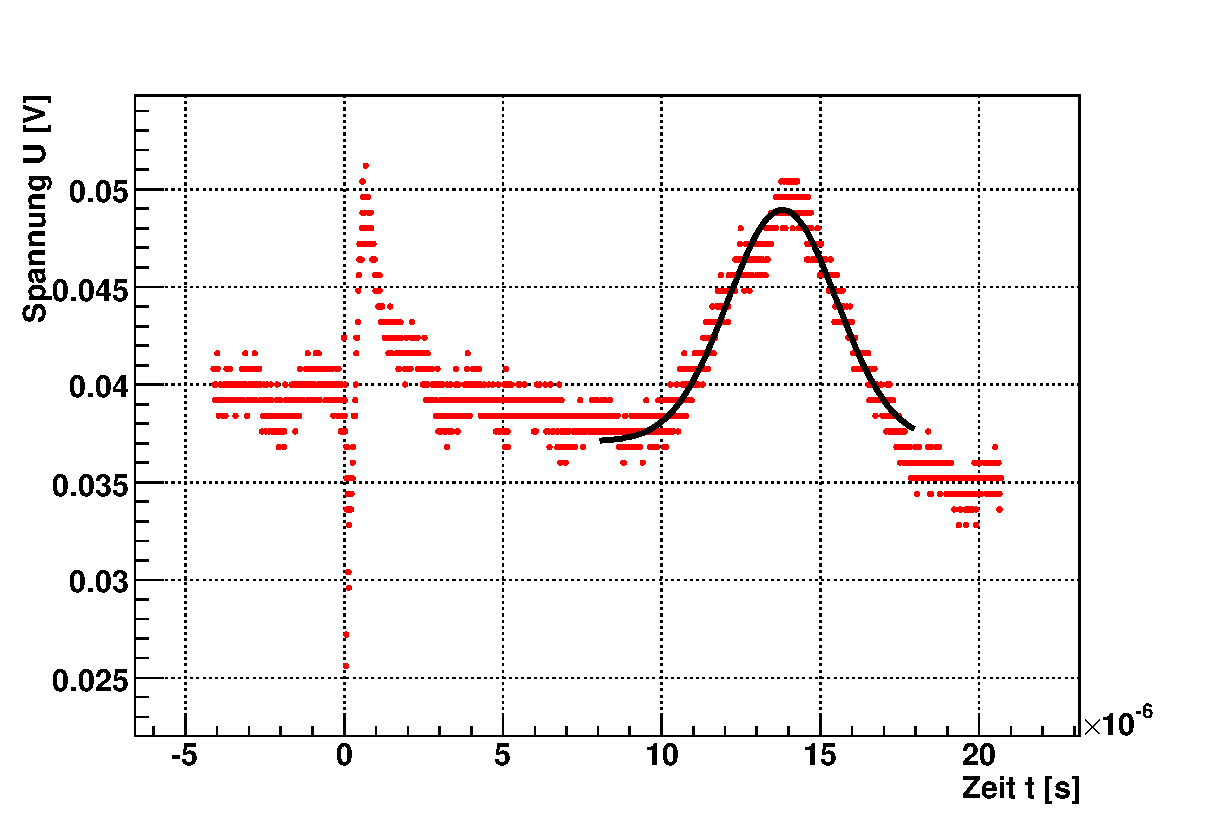
\includegraphics[width=0.9\linewidth]{pictures/varVolt/07.eps}
\small{30 V}
\end{minipage}
\begin{minipage}{0.33\linewidth}
\centering 
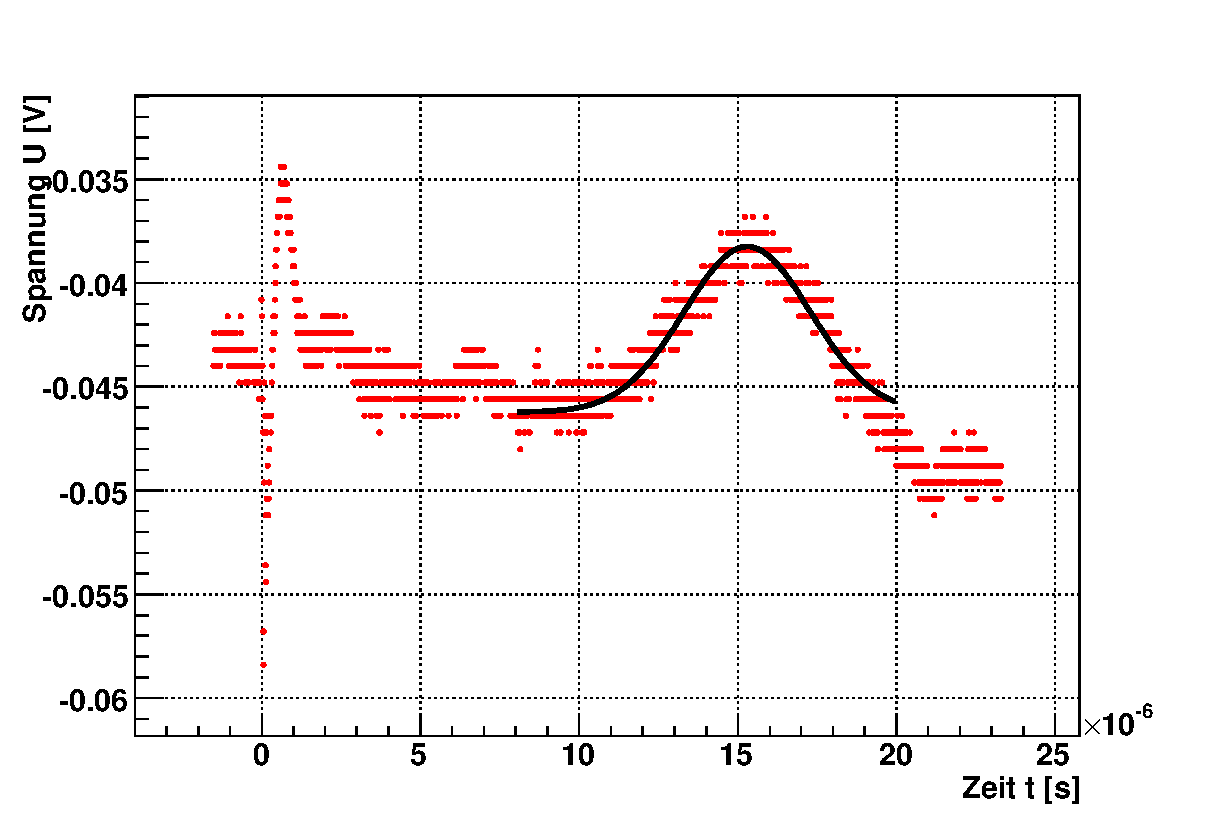
\includegraphics[width=0.9\linewidth]{pictures/varVolt/08.eps}
\small{26,8 V}
\end{minipage}
\end{figure}

\begin{figure}[H]  
\begin{minipage}{0.33\linewidth}
\centering
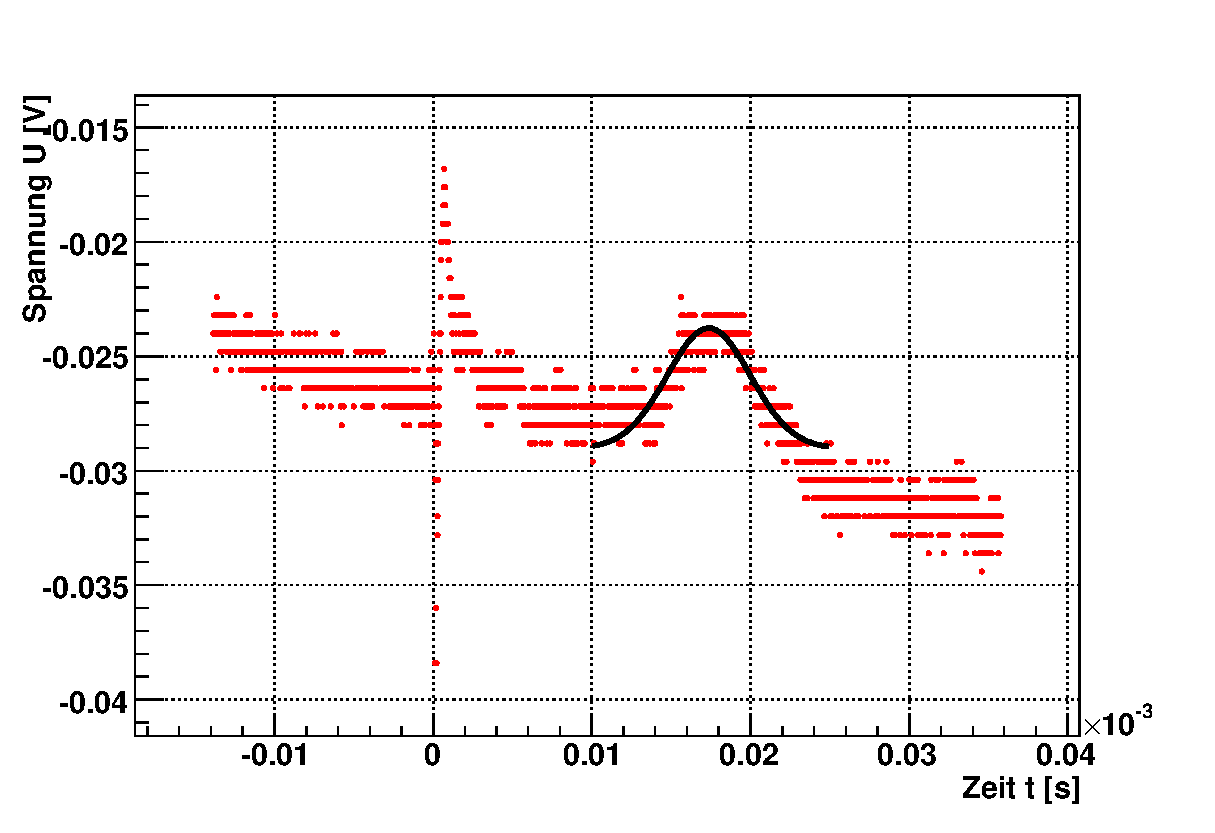
\includegraphics[width=0.9\linewidth]{pictures/varVolt/09.eps}
\small{23,2 V}
\end{minipage}
\begin{minipage}{0.33\linewidth}
\centering
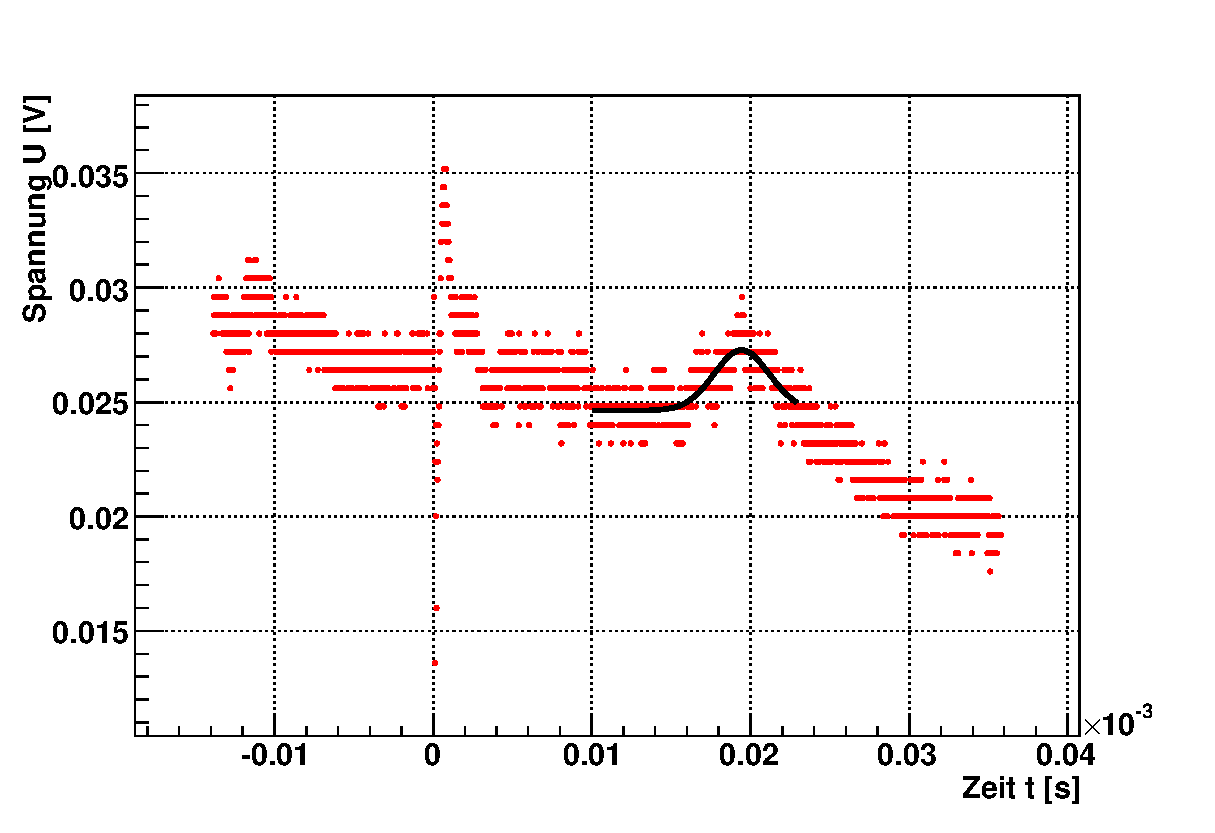
\includegraphics[width=0.9\linewidth]{pictures/varVolt/10.eps}
\small{20 V}
\end{minipage}
\begin{minipage}{0.33\linewidth}
\centering 
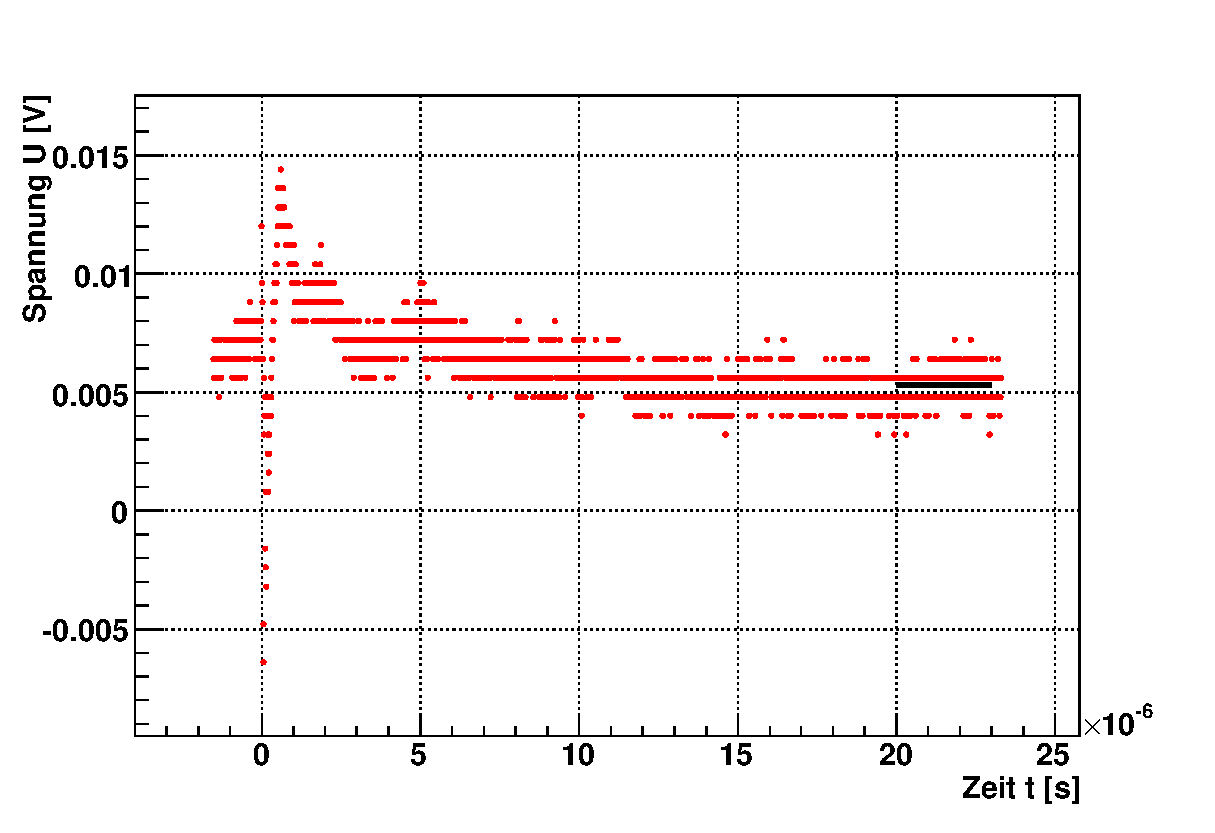
\includegraphics[width=0.9\linewidth]{pictures/varVolt/11.eps}
\small{15,2 V}
\end{minipage}
\end{figure}

\subsection{Halbleiterdetektor}
Nachdem wir leider feststellen mussten, das die von uns aufgezeichneten Daten nur Untergrund enthielten und somit für die Auswertung unbrauchbar waren, erhielten wir die Daten der Assistentin.\\

Diese Daten haben folgendes Aussehen:
\begin{figure}[H]
\centering
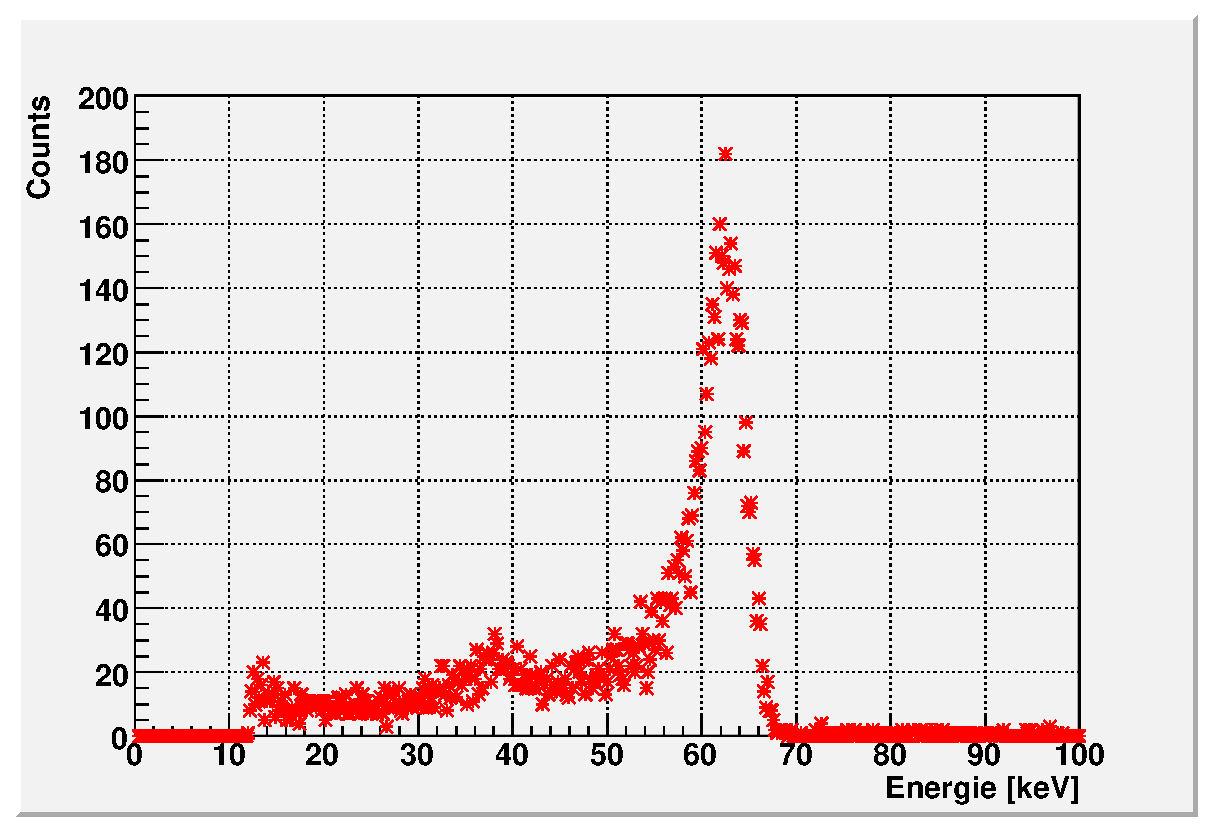
\includegraphics[width=0.9\linewidth]{pictures/gamma/scaled_cdte_am.eps}
\caption{$^{241}Am$ mit CdTe-Sonde}
\end{figure}

\begin{figure}[H]
\centering
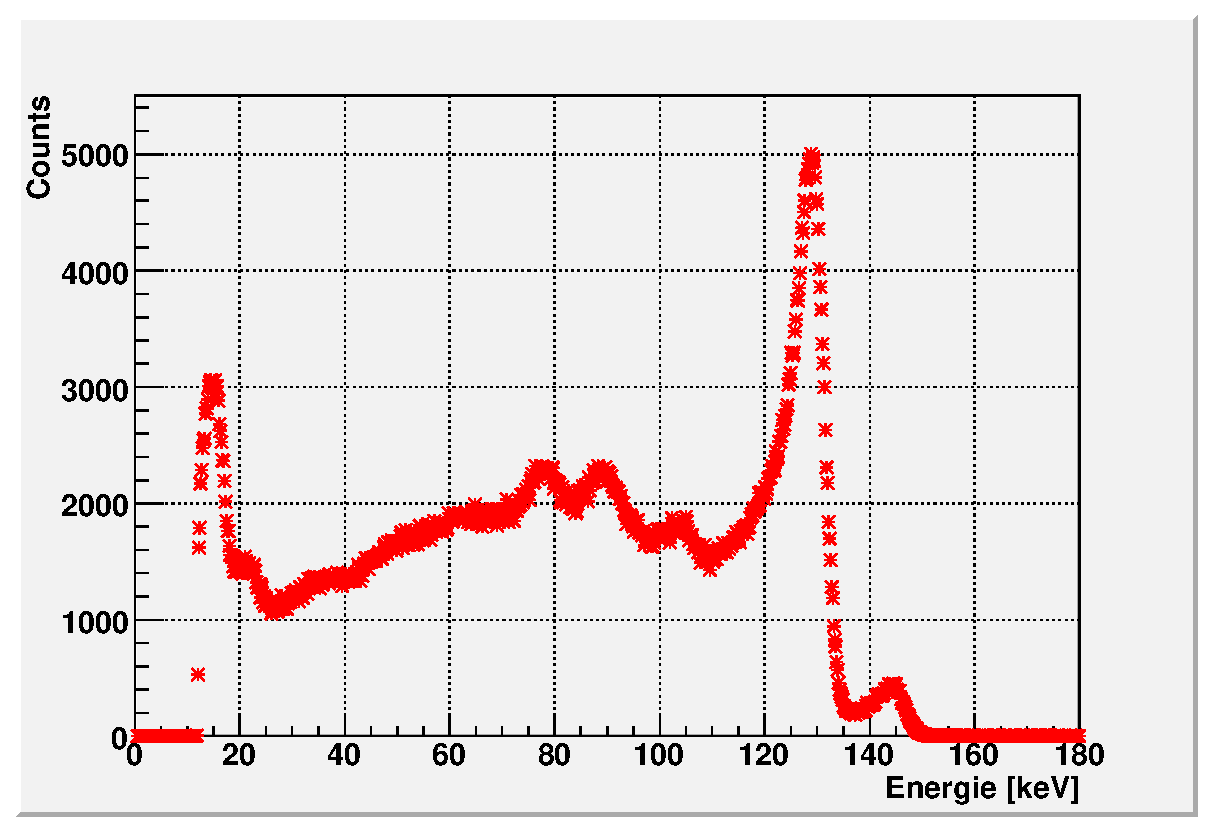
\includegraphics[width=0.9\linewidth]{pictures/gamma/scaled_cdte_co.eps}
\caption{$^{57}Co$ mit CdTe-Sonde}
\end{figure}

\begin{figure}[H]
\centering
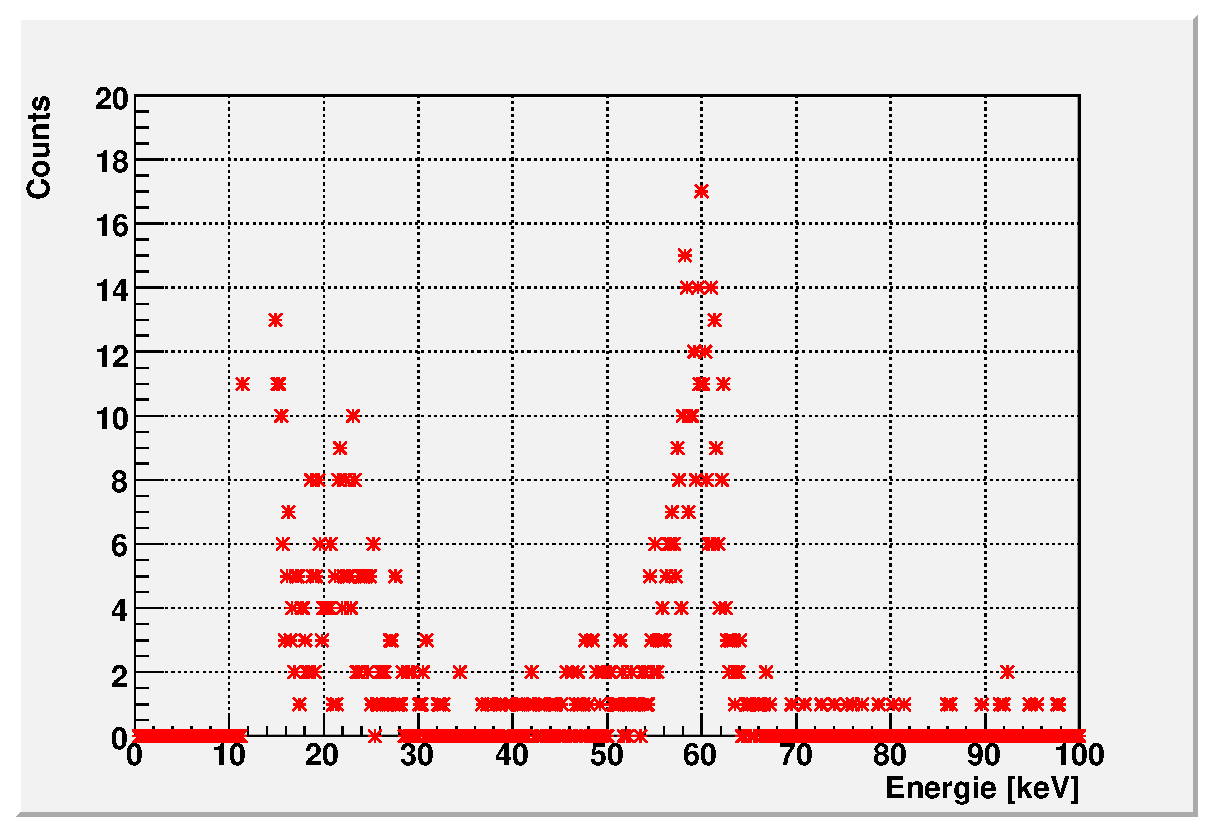
\includegraphics[width=0.9\linewidth]{pictures/gamma/scaled_si_am.eps}
\caption{$^{241}Am$ mit Silizium-Sonde}
\end{figure}

\begin{figure}[H]
\centering
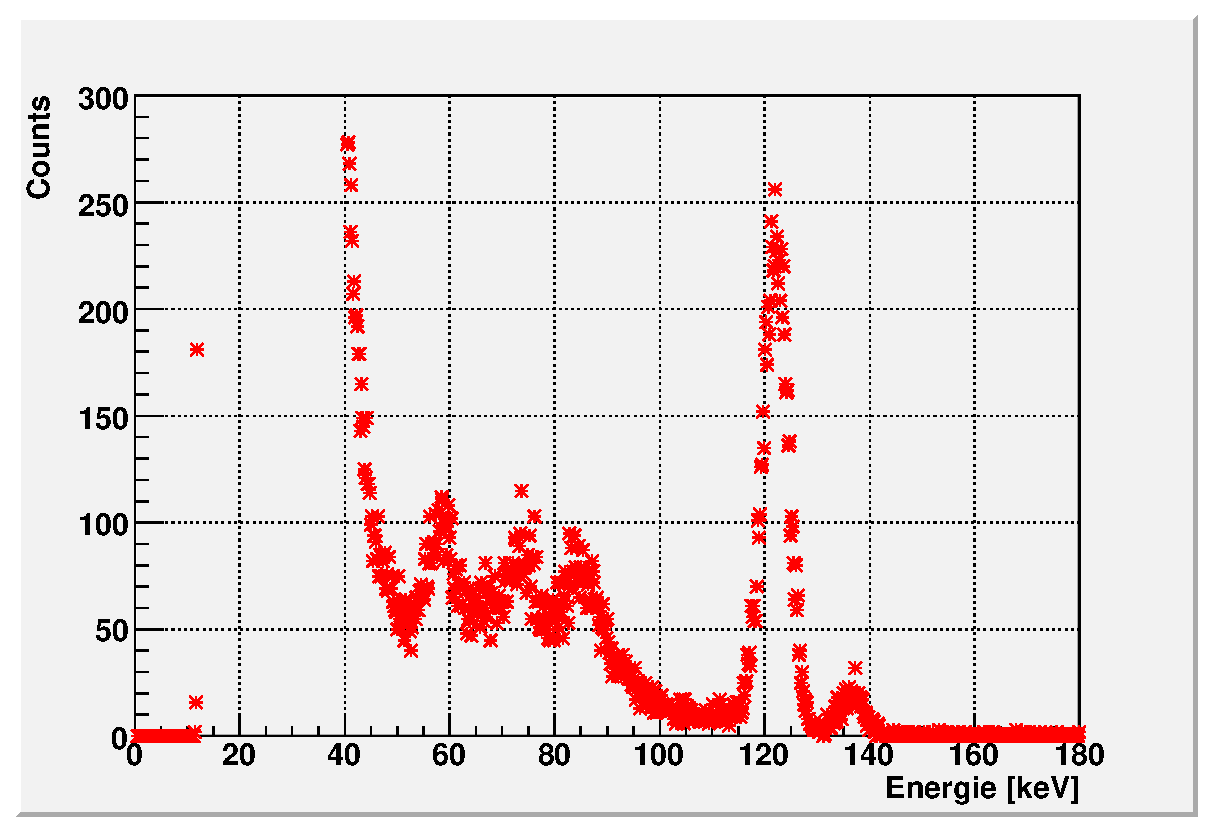
\includegraphics[width=0.9\linewidth]{pictures/gamma/scaled_si_co.eps}
\caption{$^{57}Co$ mit Silizium-Sonde}
\end{figure}

Wir identifizierten die Peaks die zu den Strahlungsquellen gehörten und fitteten entsprechende Gausskurven an diese:

\begin{figure}[H]
\centering
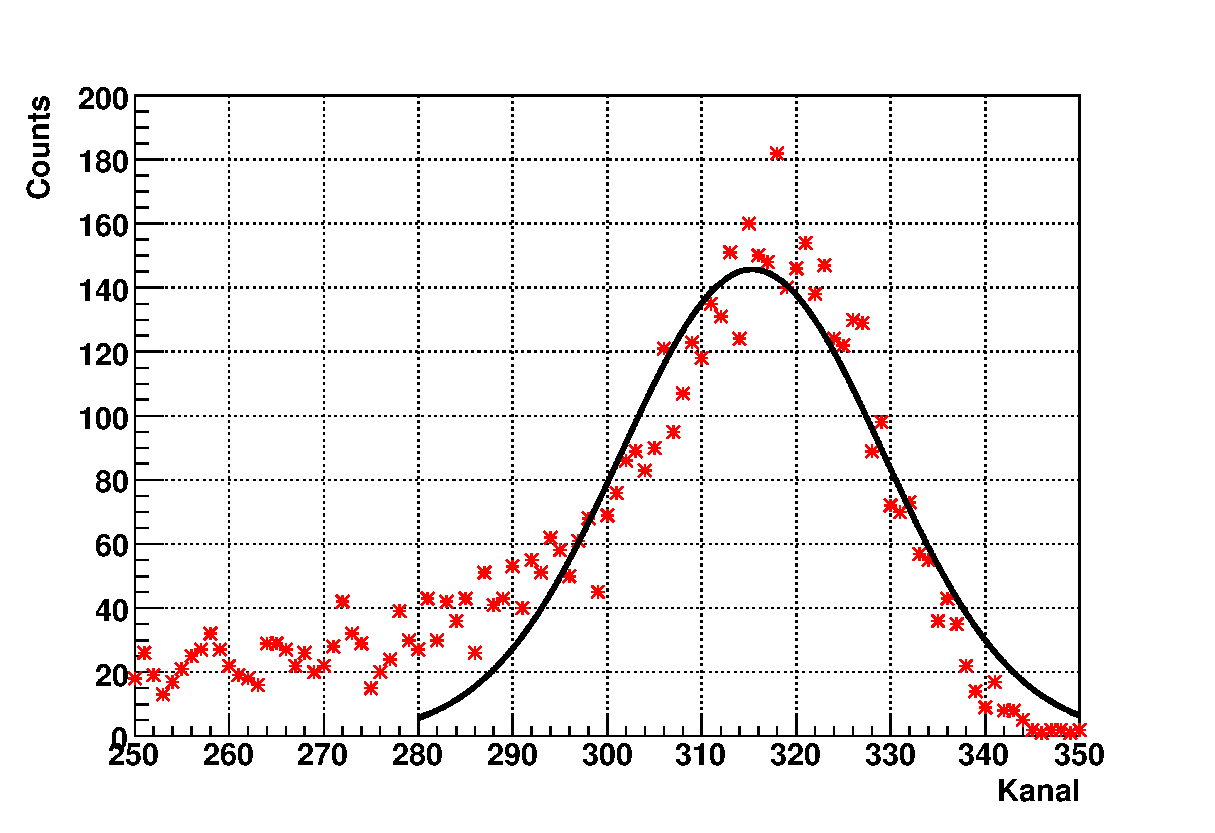
\includegraphics[width=0.9\linewidth]{../plot/eps/gamma/cdte_am.eps}
\caption{$^{241}Am$ mit CdTe-Sonde}
\end{figure}

\begin{figure}[H]
\centering
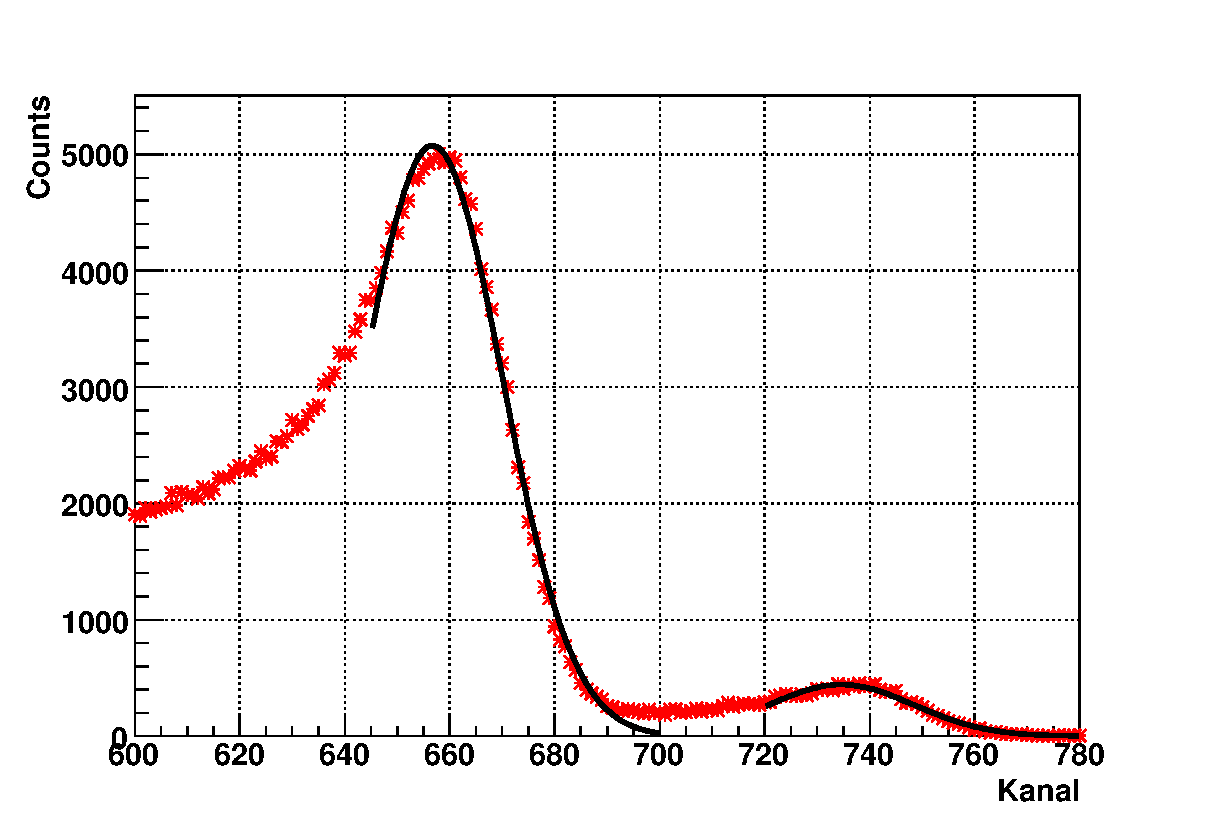
\includegraphics[width=0.9\linewidth]{../plot/eps/gamma/cdte_co.eps}
\caption{$^{57}Co$ mit CdTe-Sonde}
\end{figure}

\begin{figure}[H]
\centering
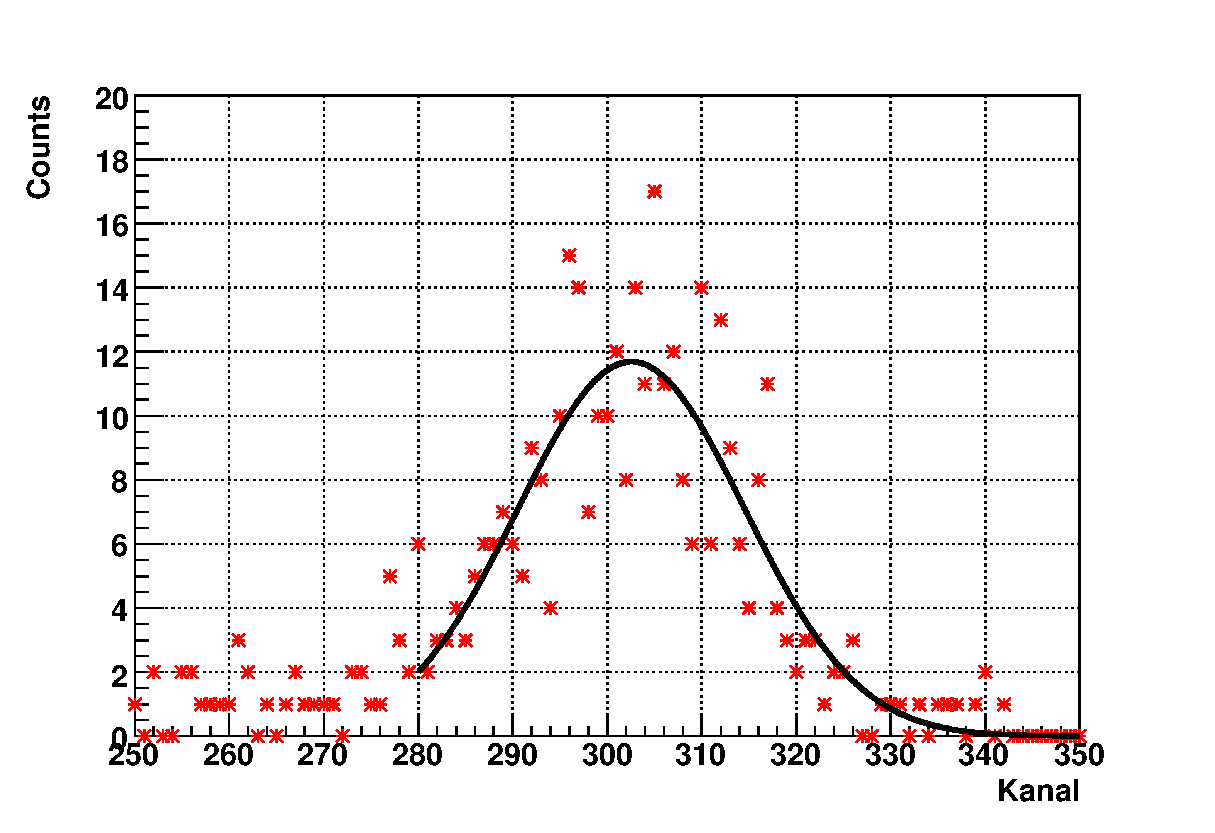
\includegraphics[width=0.9\linewidth]{../plot/eps/gamma/si_am.eps}
\caption{$^{241}Am$ mit Silizium-Sonde}
\end{figure}

\begin{figure}[H]
\centering
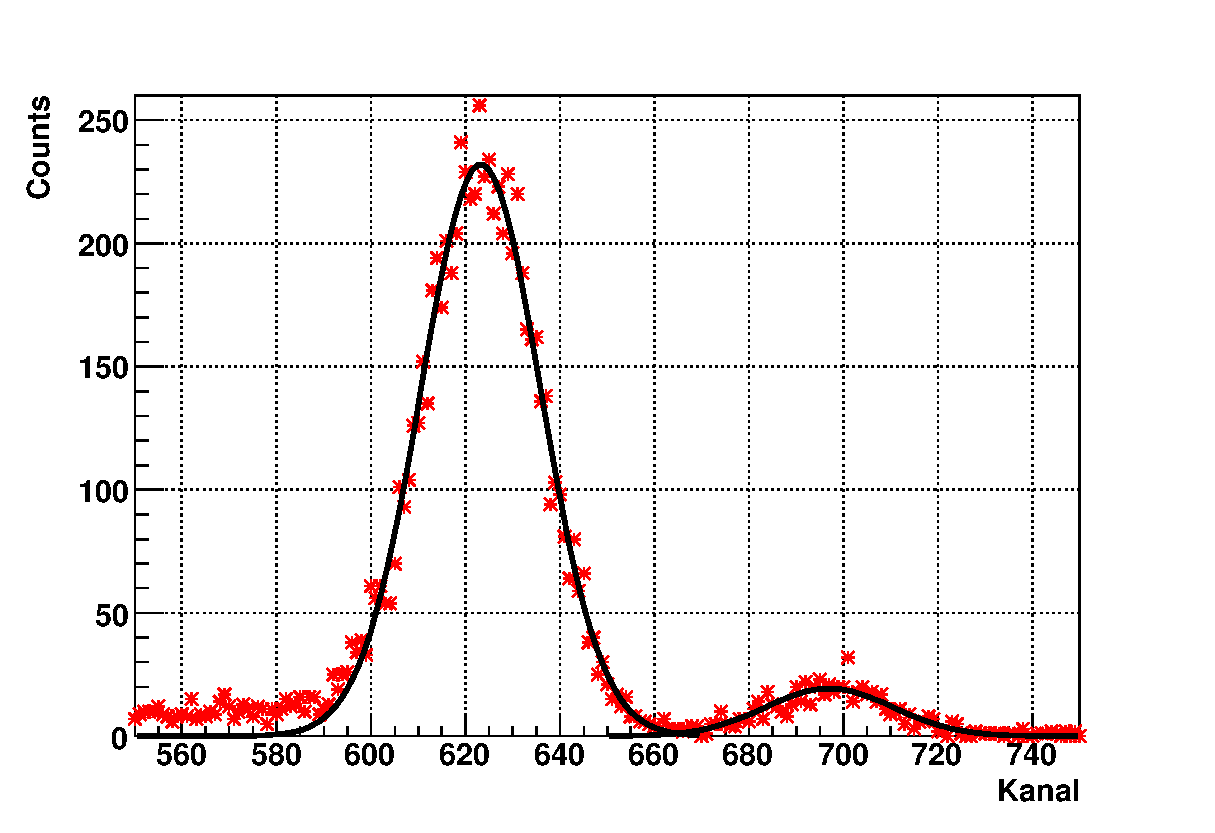
\includegraphics[width=0.9\linewidth]{../plot/eps/gamma/si_co.eps}
\caption{$^{57}Co$ mit Silizium-Sonde}
\end{figure}

Mit den Schwerpunkten und den bekannten Energien ($^{241}Am:59keV$, $^{57}Co:122$ \& $136keV$) der drei Kurven ergibt sich für jeden Sensor die Eichgerade:
\begin{figure}[H]
\centering
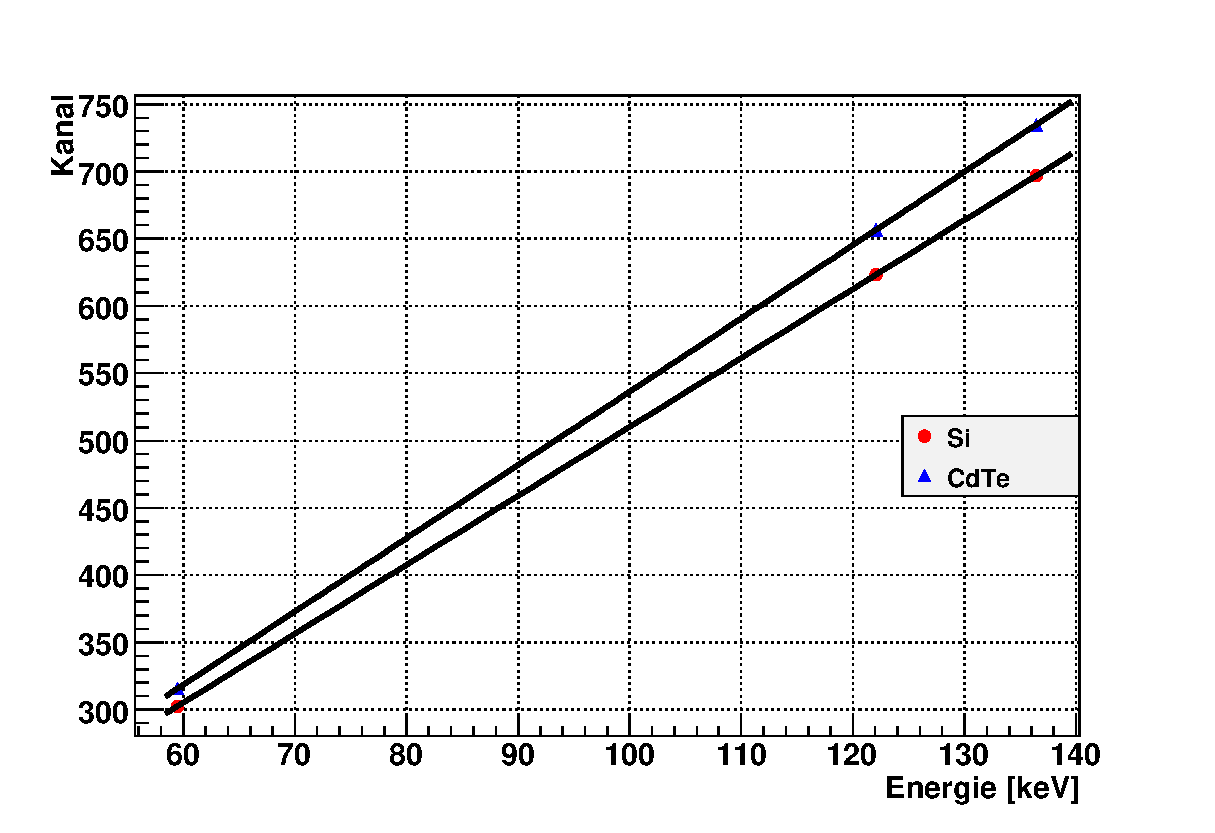
\includegraphics[width=0.9\linewidth]{../plot/eps/gamma/finalfit.eps}
\caption{Energieeichung}
\end{figure}
Hat diese die Form $a \cdot x + b$, so folgt für den Zusammenhang zwischen Enerie $E$ und Messkanal $K$:
\begin{align}
 \notag	E(K) = \frac{1}{a}(K-b)
\end{align}


\subsubsection{Absorptionsverhältnisse}
Die Zahl der aufgefangenen Photonen gibt der Faktor $C$ des Gaußfitts an:
\begin{align*}
 G(E) = C \frac{1}{\sqrt{2 \pi \sigma}} e^{-\frac{1}{2}\left(\frac{E-E_i}{\sigma_i}\right)^2}
\end{align*}
Somit lässt sich das Verhältniss der Apsorptionswahrscheinlichkeiten berechnen, hierbei muss noch beachtet werden, dass die beiden Detektoren unterschiedliche aktive Flächen haben. Der Fehler auf die Verhältnisse resultiert aus dem Fehler von $C$

\begin{center}
% use packages: array
\begin{tabular}{|l|lll|}
\hline
Absorbtionsverhältnisse \\
Energie [keV] & Litheraturwert[\%] & Messergebniss [\%] & Fehler [\%] \\
\hline
59.5 & 1.40 & 22.07 & 0.06 \\
122.04 & 1.83 & 21.83 & 0.01 \\
136.47 & 1.2 & 21.82 & 0.03 \\
\hline
\end{tabular}
\end{center}


%Absorbverhä----------------------------------------hier----------------------

\subsubsection{Relative Energieauflösung}
Die relative Energieauflösung bezeichnet das Verhältnis der Halbwertsbreite
eines Peaks zu dessen Lage. Die Halbwertsbreite einer Gaußverteilung lässt sich einfach aus der Standartabweichung berechnen:
\begin{align*}
 FWHM = 2\sqrt{2 ln 2} \sigma \approx 2,35\sigma
\end{align*}
die relative Energieauflösung wird damit zu:
\begin{align*}
 RER(E) = \frac{FWHM_E}{E} \approx \frac{2,35\sigma_E}{E}
\end{align*}

Der Fehler berechnet sich zu:
\begin{align*}
 s_{RER} = RER \cdot \sqrt{\left(\frac{s_E}{E}\right)^2 + \left(\frac{s_{\sigma}}{\sigma}\right)^2}
\end{align*}



\section{Zusammenfassung}
Hier nochmal eine Zusammenstellung der Ergebnisse und ein Fazit zu den jeweiligen Versuchsteilen:
\begin{itemize}
 \item Vermessung der Bandlücke
\begin{align*}
 E_G = 0,741 \pm 0,045 eV
\end{align*}
Verglichen mit dem Literaturwert von $E_G = 0,66 eV$ liegen wir damit in der richtigen Größenordnung. Der Literaturwert liegt in der $2\sigma$ Umgebung unseres Messwerts
\item Haynes-Shockley Experiment
Obwohl die Fits bis auf die der Breiten alle recht gut aussahen, gelang es uns nicht Werte zu erhalten mit denen man im Rahmen der Fehlergrenzen auf den Litheraturwert kommt. Trotz langer Fehleranalyse war es uns nicht möglich ihn zu finden, wesshalb wir auch diesen Teil des Auswertungsskripts angehängt haben. Desweiteren existiert auch ein SVN-Repository, in welchem die Skripte samt Pfaden und Daten abgelegt sind und man Ideen zur Korektur sofort Testen kann, die Adresse ist: \\ \url{http://fp-auswertung.googlecode.com/svn/trunk/halbleiter/}
\begin{itemize}
\item Litheraturwerte:
\begin{itemize}
 \item Beweglichkeit der Elektronen ~~~~~~~~$\mu = (0,39 \pm ?) \frac{m^2}{Vs}$ 
 \item Lebensdauer der Elektronen ~~~~~~~~~~$\tau = (45 \pm 2) \mu s $
 \item Diffusionskonstante der Elektronen ~~$D = (0,0101 \pm ?) \frac{m^2}{s}$
\end{itemize}
\item Variabler Abstand:
\begin{itemize}
 \item Beweglichkeit der Elektronen ~~~~~~~~$\mu = (0,283 \pm 0,016) \frac{m^2}{Vs}$ 
 \item Lebensdauer der Elektronen ~~~~~~~~~~$\tau = (52,2 \pm 0,3) \mu s $
 \item Diffusionskonstante der Elektronen ~~$D = (5,42 \pm 0,03) 10^{-8} \frac{m^2}{s}$
\end{itemize}
\item Variable Treiberspannung
\begin{itemize}
 \item Beweglichkeit der Elektronen ~~~~~~~~~$\mu = (111 \pm 8) \frac{m^2}{Vs}$ 
 \item Lebensdauer der Elektronen ~~~~~~~~~~~$\tau = (32,5 \pm 0,5) \mu s $
 \item Diffusionskonstante der Elektronen ~~$D = (5,53 \pm 0,06) 10^{-8} \frac{m^2}{s}$
\end{itemize}
\end{itemize}
Wie man sieht liefert unsere Analyse der Daten keine passenden Werte für die Diffusionskonstante, was der Verlauf der Breiten aber auch schon ahnen lies. Die Lebensdauer und die Beweglichkeit liegen wenigstens in der richtigen Grössenordnung, allerdings ausserhalb $2\sigma$. Unter diesen Umständen machte die Mc Kelvey Korrektur keinen Sinn.


\item Halbleiterdetektor: \\

Absorptionsverhältinisse: 
\begin{align*}
 Abs_[Si
\end{align*}
Abweichungen vom Literaturwert könne viele Ursachen haben, unteranderm wir die Absorption in den den Detektor umgebenen Schichten nicht berücksichtigt und auch die Dicke der Detektoren könnte von den Herstellerangaben abweichen.\\
\end{itemize}
Relative Energieauflösung:
%blaballslfbsl

\end{document}
